\documentclass[a4paper,12pt,oneside,openany,brazil]{abntex2}

\usepackage[T1]{fontenc}
\usepackage[utf8]{inputenc}
\usepackage[brazil]{babel}
\usepackage{geometry}
\usepackage{lmodern}
\usepackage{amsmath}
\usepackage{amssymb}
\usepackage{setspace}
\usepackage{xr-hyper}
\usepackage{hyperref}
\usepackage{xcolor}
\usepackage{graphicx}
\usepackage{placeins}
\usepackage[alf,no-abnt-option-file]{abntex2cite}
% Configuração local das citações; referências restritas às obras citadas.
\citeoption{config-citacoes-abnt}

\geometry{
    top=3cm,
    bottom=2cm,
    left=3cm,
    right=2cm
}

\setlength{\parindent}{1.25cm}
\setlength{\parskip}{0pt}
\OnehalfSpacing
\raggedbottom

% Citações indiretas: \cite{chave} ou \citeonline{chave}.
% Citações diretas curtas: ``trecho'' com \cite[p.~45]{chave},
% ou \citeonline[p.~45]{chave} antes do trecho entre aspas.
% Citações diretas com mais de três linhas: ambiente citacao, sem aspas,
% com autoria, ano e página. O espaço externo acompanha uma linha do corpo.
\setlength{\ABNTEXcitacaorecuo}{4cm}
\newlength{\espacocitacao}
\setlength{\espacocitacao}{\baselineskip}
\renewenvironment{citacao}{%
    \par\addvspace{\espacocitacao}%
    \begin{list}{}{%
        \setlength{\leftmargin}{\ABNTEXcitacaorecuo}%
        \setlength{\rightmargin}{0pt}%
        \setlength{\listparindent}{0pt}%
        \setlength{\itemindent}{0pt}%
        \setlength{\topsep}{0pt}%
        \setlength{\partopsep}{0pt}%
        \setlength{\parsep}{0pt}%
        \setlength{\itemsep}{0pt}%
    }%
    \item\relax
    \SingleSpacing\fontsize{10}{12}\selectfont
}{%
    \end{list}%
    \par\addvspace{\espacocitacao}%
}

% Numeração das seções sem o prefixo do capítulo
\renewcommand{\thesection}{\arabic{section}}
\renewcommand{\thesubsection}{\arabic{section}.\arabic{subsection}}
\renewcommand{\thesubsubsection}{\arabic{section}.\arabic{subsection}.\arabic{subsubsection}}
% O ponto pertence ao título da seção, não ao número recuperado por \ref.
\setsecnumformat{\csname the#1\endcsname\ifstrequal{#1}{section}{.}{}\quad}


\hypersetup{colorlinks=true,linkcolor=black,citecolor=black,urlcolor=black}
\renewcommand{\figurename}{Figura}

\externaldocument[M-]{manuscript_JEM}[manuscript_JEM.pdf]
\renewcommand{\thesection}{S\arabic{section}}
\renewcommand{\thetable}{S\arabic{table}}
\renewcommand{\thefigure}{S\arabic{figure}}
\renewcommand{\theequation}{S\arabic{equation}}
\renewcommand{\thesubsection}{S\arabic{section}.\arabic{subsection}}
\setsecnumformat{\ifstrequal{#1}{section}{Texto~}{}\csname the#1\endcsname\quad}
\begin{document}
\pagestyle{plain}
\aliaspagestyle{chapter}{plain}
\begin{center}
{\Large\bfseries Material suplementar}\\[0.3cm]
Preços agrícolas, capacidade produtiva e perdas anteriores na conversão da vegetação nativa em Mato Grosso\\[0.3cm]
Fernando Souza da Vieira
\end{center}
O material reúne a fundamentação ampliada, a contextualização dos dados e os procedimentos que sustentam os contrastes apresentados no manuscrito. As especificações e os resultados complementares permitem acompanhar escolhas de mensuração, composição amostral e inferência. Os Textos S1--S5 seguem esse percurso; tabelas e figuras possuem numeração própria, e as chamadas com numeração sem prefixo S remetem ao manuscrito, onde se encontram os elementos compartilhados.

\section{Fundamentos ambientais, produtivos e institucionais}
\label{text:s1}
\label{literatura}

Compreender a relação entre expansão agropecuária e conversão exige distinguir as condições em que produzir mais envolve abrir áreas ou aproveitar terras já utilizadas. Essa escolha aproxima a comparação entre retornos privados e custos ambientais das condições que tornam cada uso atraente para o produtor. A revisão parte dessa relação para examinar como preços e capacidade produtiva configuram os incentivos, como perdas anteriores podem modificar as respostas e como as instituições condicionam as alternativas disponíveis. Esse percurso fundamenta as duas proposições de H1 para a conversão agrícola, mantendo a pastagem como comparação complementar.

\subsection{Retornos privados e custos ambientais da expansão agropecuária}
\label{literatura-retornos}

A conversão pode ampliar a renda privada e reduzir serviços ambientais cujas perdas não recaem integralmente sobre quem decide converter. Ao organizar a escolha em torno das rendas relativas da agricultura e da floresta, \citeonline{Angelsen2010} permite situar esse descompasso: a produção oferece receitas apropriáveis, enquanto parte dos benefícios da vegetação é compartilhada com outros agentes. A decisão depende dos benefícios e custos das alternativas efetivamente acessíveis ao produtor, inclusive das receitas que possa obter ao conservar e das restrições à abertura. Como conservar implica renunciar ao benefício líquido da melhor alternativa acessível de uso da terra, esse benefício define o custo de oportunidade da conservação, distinto dos gastos de manutenção e das perdas ambientais impostas a terceiros. O valor da produção na área convertida constitui, portanto, apenas um componente dessa comparação.

O armazenamento e o sequestro de carbono exemplificam benefícios de alcance global que não se convertem automaticamente em renda privada \cite{Angelsen2010}, mesmo quando a conservação é remunerada, pois a receita obtida não equivale necessariamente ao valor social do serviço mantido. Avaliar esse descompasso requer delimitar a mudança biofísica antes de atribuir-lhe um valor econômico. Na Fazenda Tanguro, na transição Amazônia--Cerrado, \citeonline{Popin2025} examinaram a substituição de floresta por soja e encontraram respostas do carbono do solo diferentes conforme profundidade e manejo. O estudo caracteriza, assim, uma dimensão da mudança ambiental, cujo alcance não equivale à mensuração das emissões totais ou de seu custo social.

Ao incorporar benefícios que não se expressam na receita agrícola, a avaliação econômica da terra passa a considerar custos e benefícios que a comparação privada pode omitir. Na Amazônia brasileira, \citeonline{Mann2012} examinaram essa diferença ao avaliar o retorno potencial da soja e o valor dos serviços mantidos pela floresta. A comparação ajuda a compreender como a conversão pode permanecer atraente para o produtor e, ao mesmo tempo, impor perdas ambientais a outros agentes.

O valor atribuído à conservação depende, contudo, tanto da mensuração do estoque ambiental quanto do critério utilizado para valorá-lo. \citeonline{FerreiraEtAl2026} compararam, para um mesmo inventário em Tauari, no Acre, equações alométricas usadas para estimar biomassa a partir de medidas das árvores. Os autores mostraram que a escolha dessas equações alterou a valoração do carbono sob parâmetros contábeis constantes. O estudo distinguiu avaliação por preço de crédito e por um valor de referência para o custo social do carbono. A comparação entre estudos acrescenta diferenças nos serviços incluídos e nos métodos. Em escala nacional, \citeonline{CampoliStivali2026} harmonizaram estimativas de custo social do desmatamento nos biomas brasileiros em dólares de 2025 por hectare, evidenciando essas diferenças. Dano climático por unidade de emissão, receita de crédito e perda ambiental por hectare respondem, assim, a perguntas distintas. Essa literatura fundamenta a diferença entre benefícios privados e custos sociais, enquanto o objeto deste artigo permanece nas condições em que os incentivos se associam à conversão.

\subsection{Preços agropecuários e decisões de uso da terra}
\label{literatura-precos}

Os preços participam da comparação entre produzir em áreas já utilizadas, abrir novas áreas e conservar. Mantidos os custos e as demais condições, uma alta do preço do produto gera maior acréscimo de receita por hectare onde a produção potencial da cultura é maior, embora sua tradução em rentabilidade também dependa de fertilizantes, combustíveis, herbicidas e custos de abertura e escoamento. Uma relação de troca produto/insumo informa quanto desse insumo pode ser adquirido com a venda do produto, oferecendo uma leitura parcial dessa comparação, sem representar a cesta completa de custos ou o lucro esperado. A heterogeneidade do incentivo de receita motiva H1a, mas não demonstra o sinal da associação com a conversão, pois a resposta pode ocorrer em terras já utilizadas e depende dos custos, das restrições e das parcelas disponíveis. A hipótese constitui, assim, uma conjectura empírica condicional sobre como essa heterogeneidade aparece na conversão agrícola.

Os atributos dos territórios ajudam a compreender por que uma mesma cotação pode se relacionar de formas distintas com o uso da terra. Nos Estados Unidos, \citeonline{LubowskiEtAl2008} estimaram decisões considerando retornos líquidos e qualidade da terra, enquanto, na Amazônia, \citeonline{Pfaff1999} relacionou desmatamento, características locais e custos de transporte. A relevância de solos, precipitação, acesso a mercados e proteção territorial também foi documentada por \citeonline{ChomitzThomas2003}. Em contextos distintos, esses estudos mostram que o preço de venda precisa ser interpretado junto às possibilidades de produção e aos custos de realizá-la, conjunto no qual a capacidade produtiva integra o incentivo sem substituir as demais condições.

Para representar essas possibilidades, é necessário distinguir o rendimento realizado, que incorpora manejo, insumos e seleção das parcelas cultivadas, do potencial produtivo definido sob um cenário padronizado. A interação desse potencial com os preços aproxima os incentivos de receita, sem constituir uma conta monetária observada de receita ou lucro. A capacidade potencial caracteriza diferenças nas possibilidades produtivas entre localidades, enquanto a identificação de perdas exige comparar o desempenho realizado com uma referência histórica local. A escolha de uma medida fixa no painel tampouco garante exogeneidade ou anterioridade de todos os seus componentes às decisões analisadas, condições que precisam ser consideradas ao passar do mecanismo econômico à comparação empírica.

A exposição a uma cotação comum foi examinada por \citeonline{BermanEtAl2023} ao combinar preços internacionais e aptidão agrícola em escala tropical, entre 2001 e 2018. Os autores encontraram associação positiva com desmatamento, heterogênea conforme condições econômicas locais, oferecendo uma referência para a pergunta sobre diferenças municipais em Mato Grosso. O presente artigo emprega rendimentos potenciais de soja e milho e taxas de conversão da vegetação nativa por destino, medidas distintas do índice composto de preços ponderados pela aptidão e da perda florestal do estudo tropical. A aplicação dessa lógica de exposição exige, portanto, condições próprias de inferência: preços podem refletir choques de oferta, e o potencial padronizado não elimina fatores omitidos que variam no tempo, de modo que nem as magnitudes nem a identificação daquele estudo são transferidas ao painel municipal.

Além de distinguir as condições de exposição aos preços, é preciso considerar o uso que se expande e aquele que é substituído. Na bacia do Tapajós, \citeonline{Braganca2018} encontrou que a valorização das lavouras em relação à carne favoreceu a substituição de pastagens por cultivos e reduziu o desmatamento local, resultado condicionado pelos custos e pelas possibilidades de realocação dos fatores, e não uma consequência necessária dessa substituição. Na porção florestal de Mato Grosso, 91\% da expansão da soja entre 2006 e 2010 ocorreu em terras anteriormente abertas, sobretudo pastagens, enquanto novas pastagens responderam pela maior parte do desmatamento remanescente \cite{MacedoEtAl2012}. Esses antecedentes mostram por que a valorização agrícola pode estimular a reorganização de áreas abertas ao mesmo tempo em que a conversão persiste para outro destino, tornando necessário separar crescimento produtivo, substituição entre usos e abertura de novas áreas.

As condições tecnológicas ampliam as alternativas em terras já utilizadas. \citeonline{Spera2017} destacou cultivares, correção dos solos e ciclos curtos que viabilizam soja e milho no mesmo ano, enquanto \citeonline{VanWeyEtAl2013} associaram duas safras a transportes, produção anterior e conexão com mercados. Essas possibilidades de produzir se articulam às condições de comercialização: \citeonline{LathuilliereEtAl2014} documentaram que, entre 2006 e 2010, a China superou a Europa como destino da soja exportada por Mato Grosso. As evidências situam a expansão em um contexto de mudanças nas possibilidades de produzir e vender, sem identificar, isoladamente, um choque exógeno de demanda ou assegurar que ganhos de rendimento sempre resultem em conservação.

A evolução produtiva também precisa ser considerada ao caracterizar as quebras de safra. Uma redução da produção total pode decorrer de menor área plantada, sem representar perda por hectare, e um rendimento inferior ao potencial padronizado pode refletir condições persistentes de manejo. No presente artigo, as quebras são aproximadas por desvios negativos da produção por hectare plantado em relação a uma referência construída com o histórico anterior, considerando a evolução produtiva local. Essa razão reúne o rendimento na área colhida e a proporção da área plantada que chegou à colheita, permitindo considerar perdas que o rendimento por hectare colhido, isoladamente, pode omitir. Ainda assim, mudanças nos insumos e na composição das parcelas cultivadas também afetam essa medida, que não identifica por si só a origem da perda.

Uma perda que reduza os recursos próprios disponíveis pode limitar o financiamento da produção e da abertura de áreas. Há evidência de que condições financeiras afetam decisões agrícolas, mas seu alcance depende da atividade e da restrição examinada. Na Amazônia brasileira, \citeonline{AssuncaoEtAl2020Credito} estimaram redução do desmatamento após o condicionamento do crédito rural à regularidade fundiária e ambiental, com efeito mais evidente em municípios voltados à pecuária e estimativa imprecisa nos voltados às lavouras. Em experimentos no norte de Gana, \citeonline{KarlanEtAl2014} encontraram aumento do investimento agrícola com a oferta de seguro, destacando o risco não segurado como restrição distinta da falta de capital. Esses resultados sustentam a relevância do financiamento e do risco, mas não demonstram que uma quebra de soja ou milho em Mato Grosso reduza recursos e, por essa via, a conversão subsequente.

A expansão territorial também foi observada após choques produtivos adversos. Na Zâmbia, \citeonline{OrdonezEtAl2025} examinaram uma infestação de lagarta-do-cartucho do milho e encontraram perdas produtivas, aumento da produção de carvão e expansão de lavouras. Esta última resposta foi imprecisa no painel de famílias, mas apareceu na análise espacial, de modo que as evidências de extração e expansão não devem ser confundidas. Em um texto para discussão baseado em dados globais e censos agropecuários brasileiros, \citeonline{HsiaoEtAl2026} relacionaram calor extremo, perda florestal e expansão de lavouras. Para o Brasil, encontraram redução da produtividade física acompanhada de aumento dos preços agrícolas locais, evidência compatível com um canal de preços na resposta territorial. Os dois estudos mostram que perdas produtivas podem ser acompanhadas de expansão, sob condições próprias de mercado e acesso a recursos. Seus resultados não estabelecem uma intenção compensatória comum aos produtores nem se transferem diretamente ao contraste municipal de soja e milho com cotações internacionais.

Essas possibilidades motivam H1b: perdas anteriores podem modificar a associação entre preços e conversão, sem determinar previamente o sinal dessa modificação. A restrição de recursos poderia limitar a capacidade de responder a uma valorização, enquanto a busca de recomposição da produção poderia favorecer a expansão quando houvesse terra e financiamento acessíveis. São hipóteses explicativas para a relação investigada, e não mecanismos demonstrados neste artigo. Uma perda física tampouco equivale necessariamente a queda de receita ou de lucro, pois preços, custos e condições de comercialização também participam dessa comparação. O contraste proposto examina se a associação preço--conversão varia com a ocorrência e a intensidade das perdas anteriores, mediante a interação entre preços e perdas, sem identificar isoladamente esses canais. A ordenação temporal é necessária à interpretação, mas a presença de defasagens não demonstra expectativas ou planejamento intertemporal.

A literatura fundamenta, assim, o exame da associação preço--conversão conforme a capacidade potencial e as perdas anteriores, preservando a distinção entre as duas sub-hipóteses. A pastagem permite comparar destinos, sem receber o mesmo sinal previsto para a heterogeneidade agrícola de H1a. O preço da carne contextualiza incentivos relativos, mas o potencial de soja e milho não representa produtividade pecuária.

\subsection{Ambiente institucional e respostas aos incentivos econômicos}
\label{literatura-instituicoes}

As instituições condicionam essas alternativas ao modificar o que os agentes podem fazer e os custos de cada escolha. A distinção de \citeonline{North1991} entre regras formais e restrições informais, complementada pela separação entre regras e organizações em \citeonline{North1993}, ajuda a reconhecer que a existência de uma norma não equivale à sua implementação. É nessa passagem às regras efetivamente praticadas que \citeonline{Ostrom2009} situa o monitoramento e as sanções na governança dos recursos naturais, cuja relação com o cumprimento ambiental foi examinada por \citeonline{Shimshack2014}. O condicionamento institucional envolve, portanto, tanto o conteúdo das restrições quanto as condições em que elas alteram o retorno esperado de descumpri-las.

As regras de acesso à terra podem alterar oportunidades produtivas, além de impor restrições. \citeonline{PachecoMeyer2022} compararam regimes fundiários e encontraram resultados que variaram com a origem, a alternativa de destinação e o contexto. \citeonline{ProbstEtAl2020} observaram aumento do desmatamento entre pequenos e médios proprietários titulados pelo Terra Legal e maior resposta aos preços. Esses resultados qualificam a interpretação da regularização: sua relação com a conservação depende de como modifica as alternativas do produtor, e não apenas da existência de um título.

O cadastro ambiental também pode alterar as oportunidades produtivas ao se relacionar com o acesso a financiamento. No Pará e em Mato Grosso, \citeonline{JungEtAl2022} examinaram o CAR com procedimentos para mitigar seleção e encontraram expansão de pastagens, heterogênea por porte e conformidade ambiental, sem efeito estatisticamente significativo sobre a área de lavouras. A ausência de significância não demonstra efeito exatamente zero, e essas medidas de uso da terra não devem ser equiparadas automaticamente às transições brutas examinadas neste artigo. As evidências compatíveis com um canal de crédito situam o cadastro também entre as condições de financiamento da produção, mostrando por que seu papel não se esgota na exigência ambiental. Essa relação pode ser pertinente às alternativas disponíveis após uma perda, embora o estudo não identifique a mediação do crédito entre quebras de safra e conversão.

Além das condições de acesso à produção, as instituições podem modificar os custos esperados do descumprimento por meio de monitoramento e sanções. \citeonline{AssuncaoEtAl2023} exploraram limitações de detecção por nuvens no DETER e identificaram contenção do desmatamento, enquanto \citeonline{Sousa2016} examinou dificuldades de aplicação de sanções em Mato Grosso. Esses estudos permitem distinguir a existência de instrumentos, sua implementação e seus efeitos, dimensões que uma única contagem administrativa não consegue representar conjuntamente.

As restrições comerciais operam pelo acesso a compradores. Ao avaliar a Moratória da Soja, \citeonline{HeilmayrEtAl2020} estimaram redução do desmatamento em áreas aptas à soja no bioma Amazônia, mediante uma comparação entre períodos, biomas e aptidão. \citeonline{HardingEtAl2021}, por sua vez, examinaram como a resposta do desmatamento aos preços variou sob diferentes instrumentos, incluindo a Moratória. Seus resultados foram compatíveis com substituição entre culturas e deslocamento da pressão para terras não protegidas. O efeito médio atribuído à política e a alteração da sensibilidade aos preços respondem a perguntas distintas. Ambos os contrastes mostram a necessidade de considerar as alternativas disponíveis ao interpretar uma restrição, sem conferir ao presente artigo identificação automática dos efeitos de cada instrumento.

A possibilidade de responder às restrições também depende dos custos de adequação e de incentivos à conservação, cuja complementaridade foi examinada por \citeonline{SticklerEtAl2013}. O Código Florestal estabelece obrigações de proteção e recomposição da vegetação nos imóveis \cite{Brasil2012}, enquanto a Moratória condiciona a comercialização da soja produzida em áreas desmatadas no bioma Amazônia segundo os critérios do acordo. Essas diferenças exigem distinguir abrangência, calendário e implementação, sem atribuir uma exposição uniforme a todos os municípios ou tomar diferenças entre biomas como efeitos das políticas. Os registros de autuação e os termos de embargo do IBAMA aproximam uma parte da atuação administrativa e podem responder às próprias infrações, de modo que não medem diretamente probabilidade de punição ou efetividade. Esses condicionantes situam a associação entre preços, capacidade, perdas anteriores e conversão, preservando a diferença entre os mecanismos discutidos na literatura e o alcance dos indicadores disponíveis.

\subsection{Síntese da literatura e implicações para a análise}
\label{literatura-sintese}

As possibilidades produtivas e as restrições discutidas na revisão se apresentam em territórios com trajetórias distintas de ocupação. Em mapas anuais de Mato Grosso entre 2001 e 2017, \citeonline{SimoesEtAl2020} registraram expansão das lavouras e das duas safras e crescimento das pastagens sobretudo ao norte, no bioma Amazônia. No Pantanal brasileiro, incluindo áreas fora do estado, \citeonline{SeidlEtAl2001} examinaram incentivos à expansão de pastagens cultivadas. Esses recortes mostram por que a comparação de usos precisa ser situada no território, em vez de tratar a expansão agropecuária como uma resposta homogênea aos incentivos.

A literatura permite, assim, formular uma comparação em que preços alteram incentivos de receita, mas sua tradução em conversão depende de possibilidades produtivas, custos, alternativas em áreas abertas e restrições. H1a examina se a associação é mais positiva onde a capacidade potencial da respectiva cultura é maior. H1b examina se perdas anteriores modificam essa associação, com sinal indeterminado. A participação do ambiente no processo econômico, a importância das condições locais e a dimensão temporal das decisões fundamentam essa comparação, sem que o desenho teste todos os mecanismos pelos quais essas dimensões podem atuar.

A contribuição articula a exposição preços--capacidade presente em Berman, a distinção de respostas de uso da terra examinada por Jung e a discussão de choques produtivos e expansão desenvolvida por Ordóñez e Hsiao. O artigo investiga essas relações em uma base municipal comum para Mato Grosso, distinguindo potenciais e perdas de soja e milho e considerando os biomas, o alcance territorial potencial da Moratória e os limites da mensuração institucional. Seu contraste se refere à associação entre preços reais e taxas de conversão bruta para agricultura, modificada pelas condições produtivas, e à comparação complementar com pastagens. Esses destinos designam os usos imediatos da área aberta, sem identificar a cultura que motivou a conversão ou uma intenção individual de compensar perdas. A seção seguinte situa essa comparação em Mato Grosso e apresenta as medidas e a cobertura necessárias à análise.


\section{Contextualização ampliada e cobertura dos dados}
\label{text:s2}
\label{descritiva-dados}

\begingroup
\newcommand{\Hobs}{3.384}
\newcommand{\Hvalid}{2.772}
\newcommand{\Hmissing}{612}
\newcommand{\HmissingPct}{18,1}
\newcommand{\Hfixed}{95}
\newcommand{\HminFracExcl}{99,8713}
\newcommand{\HfixedObs}{2.280}
\newcommand{\Hmixed}{63}
\newcommand{\HnMin}{108}
\newcommand{\HnMax}{136}
\newcommand{\HpastShare}{91,6}
\newcommand{\HagFirst}{0,16}
\newcommand{\HagLast}{0,02}
\newcommand{\HpaFirst}{1,07}
\newcommand{\HpaLast}{0,51}
\newcommand{\HibValid}{1.760}
\newcommand{\HibComplete}{1.526}
\newcommand{\HibMin}{5}
\newcommand{\HibMax}{102}
\newcommand{\HmaxAg}{8,00}
\newcommand{\HmaxPa}{26,54}


A expansão da produção agropecuária pode envolver maior aproveitamento das terras já utilizadas ou abertura de novas áreas, alternativas que dependem das condições produtivas e institucionais dos territórios. Para situar essa comparação em Mato Grosso, a seção confronta as trajetórias de produção e comércio com a conversão da vegetação e, a partir desse quadro, examina preços, autuações, capacidade potencial e perdas produtivas anteriores. A questão é como os incentivos se relacionam com a conversão sob condições locais e trajetórias produtivas distintas, sem tomar o crescimento da oferta como medida da abertura de áreas.

As informações sobre conversão abrangem 2001 a 2024 e são organizadas em uma grade de 141 municípios da malha IBGE 2023\footnote{Boa Esperança do Norte não constitui unidade autônoma na grade adotada.}. A grade permite reunir as fontes por município, mas não assegura limites históricos constantes, e a cobertura efetiva varia entre indicadores. Os grupos com informação completa de produção, conversão, autuação e perdas anteriores não constituem, portanto, uma única amostra fixa. Para construir as referências produtivas, utiliza-se também o histórico da PAM a partir de 1988, respeitando as rupturas territoriais identificadas.

\subsection{Expansão agropecuária e transformação da cobertura vegetal}
\label{descritiva-retornos}

A inserção da produção estadual nos mercados externos, inclusive a demanda chinesa discutida por \citeonline{fearnside2016china}, compõe o contexto econômico da expansão agropecuária. Essa inserção amplia a pertinência de examinar como a produção cresceu, antes de confrontá-la com a transformação da cobertura vegetal. Mais produto pode resultar de maior área colhida, de aumento da quantidade obtida por hectare ou da combinação de ambos, sem que essas mudanças correspondam à mesma pressão por novas terras.

A Figura~\ref{fig:h1-lavouras} permite distinguir essas possibilidades com dados da Produção Agrícola Municipal (PAM), do IBGE. Soja ocupa a coluna esquerda e milho, a direita. De cima para baixo, os painéis mostram área plantada, área colhida, produção e rendimento. As áreas estão em milhões de hectares; a produção, em milhões de toneladas; e o rendimento, em toneladas por hectare colhido. A área plantada corresponde à superfície semeada, enquanto a colhida registra aquela em que a colheita ocorreu.

A linha azul acompanha grupos fixos de 66 municípios para soja e 121 para milho, com registros numéricos de área plantada, colhida e produção nos 24 anos. A cinza tracejada acrescenta os municípios com informação no ano, mas incompleta no período. O grupo fixo exige continuidade dos registros de cultivo, de modo que anos sem cultivo publicado também impedem a inclusão nessa série. Nos três primeiros pares de painéis, cada ponto corresponde à soma das áreas ou da produção do grupo. Nos painéis inferiores, o rendimento é a razão entre a produção total e a área colhida total, e não a média simples dos rendimentos municipais. As curvas quase se sobrepõem nesses painéis, indicando rendimentos agregados próximos nos dois grupos.

A leitura conjunta de área colhida e rendimento revela diferenças na composição desse crescimento. Na amostra fixa de soja, o rendimento passou de 3,06 t/ha em 2001 para 3,10 em 2024, de modo que a expansão produtiva entre os extremos acompanhou principalmente a área colhida. No milho, o rendimento passou de 3,26 para 6,72 t/ha, de modo que o crescimento da produção combinou mais hectares colhidos com maior quantidade produzida em cada hectare. As duas trajetórias situam margens distintas de aumento da oferta, cujo vínculo com a abertura de áreas precisa ser examinado separadamente.

\begin{figure}[htbp]
    \centering
    % O título é apresentado pelo LaTeX, sem duplicação dentro da imagem.
    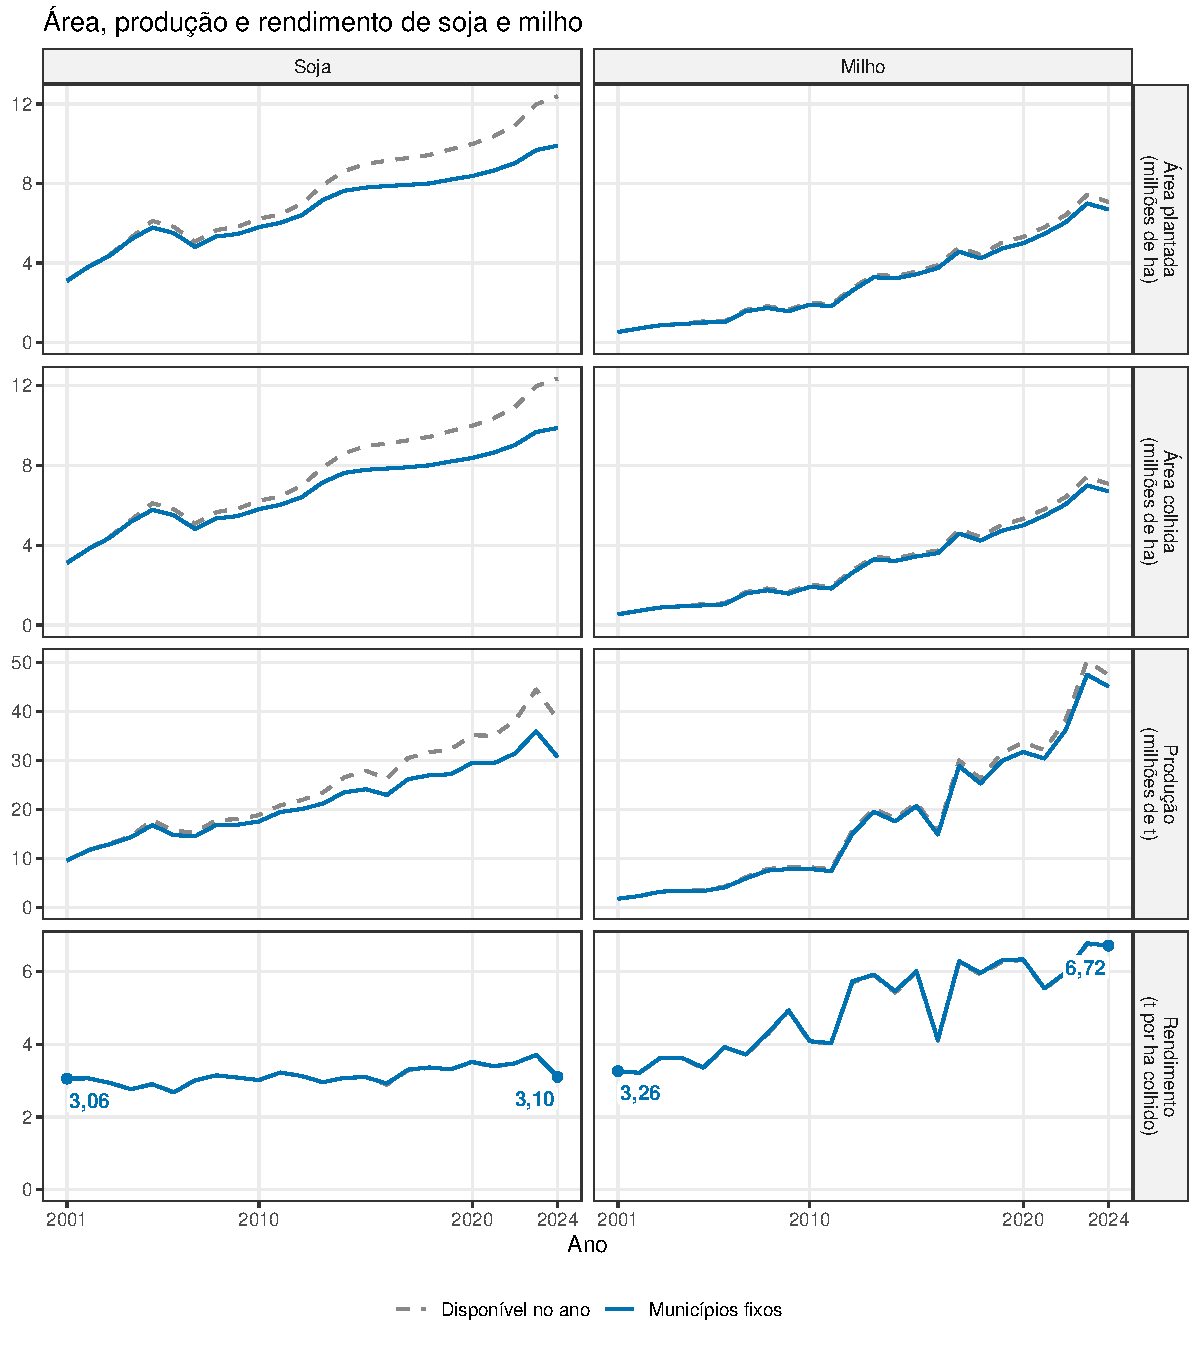
\includegraphics[width=\textwidth,trim=0 0 0 20bp,clip]{assets/fig05_lavouras.pdf}
    \caption{Evolução das lavouras de soja e milho em Mato Grosso, 2001-2024}
    \label{fig:h1-lavouras}
    \begin{minipage}{\textwidth}\footnotesize
    \centering
    Fonte: elaboração própria, com base em IBGE/PAM.

    \end{minipage}
\end{figure}
\FloatBarrier

A expansão das lavouras foi acompanhada pelo crescimento da pecuária e das vendas externas, ampliando o quadro da inserção produtiva de Mato Grosso nos mercados. A integração comercial discutida por \citeonline{LathuilliereEtAl2014} ganha, na Tabela~\ref{tab:h1-oferta-contexto}, uma caracterização complementar por estoques de animais, fluxo de abate e exportações. O rebanho soma 139 municípios com informação nos 24 anos. Abate e peso das carcaças são totais estaduais sob inspeção, somados nos quatro trimestres sem duplicação, e não produção municipal de carne.

As exportações somam registros por domicílio fiscal em Mato Grosso, nos códigos do Sistema Harmonizado a quatro dígitos (SH4): 1201 (soja), 1005 (milho) e 0201/0202 (carne bovina). Os valores FOB (\textit{Free on Board}), que excluem frete e seguro internacionais, estão em dólares correntes, sem deflação, e variam com preços, quantidades e cobertura. Entre 2001 e 2024, os municípios com registros passaram de 8 para 53 na soja, de 2 para 53 no milho e de 6 para 20 na carne.

\begin{table}[htbp]
\centering
\small
\captionstyle{\centering}
\normalcaption
\caption{Pecuária e exportações em Mato Grosso -- 2001 e 2024}
\label{tab:h1-oferta-contexto}
\begin{tabular}{lrr}
\hline
Indicador & 2001 & 2024 \\
\hline
\multicolumn{3}{l}{\textit{Pecuária}} \\
Rebanho (milhões de cabeças) & 19,92 & 32,77 \\
Abate sob inspeção (milhões de cabeças) & 2,06 & 7,14 \\
Peso de carcaças (milhões de t) & 0,51 & 1,96 \\
\hline
\multicolumn{3}{l}{\textit{Exportações FOB (US\$ milhões correntes)}} \\
Soja & 503,67 & 9.879,09 \\
Milho & 0,21 & 5.092,68 \\
Carne bovina & 5,67 & 2.308,26 \\
\hline
\end{tabular}
\par\smallskip\begin{minipage}{\textwidth}\footnotesize
\centering
Fontes: IBGE/PPM; IBGE, Pesquisa Trimestral do Abate; MDIC/SECEX, Comex Stat.
\end{minipage}
\end{table}

\FloatBarrier

Esse crescimento produtivo e comercial precisa ser confrontado com a parcela da vegetação que deu lugar a usos agropecuários. A Figura~\ref{M-fig:h1-conversao} apresenta conversão bruta para agricultura acima e para pastagem abaixo. Em cada ano e grupo, soma-se a área de vegetação convertida para o destino e divide-se pela soma da vegetação disponível no início do período, em porcentagem. Numerador e denominador usam os mesmos municípios e cobertura espacial. A taxa agregada é uma razão de somas, distinta da média das taxas municipais. Esses fluxos registram transições entre mapas consecutivos, e não diferenças líquidas entre os estoques de vegetação, que também podem incorporar transições em sentido contrário.

Dos \Hobs{} pares município--ano da grade, \Hvalid{} têm conversão observada. A linha azul acompanha os \Hfixed{} municípios com informação nos 24 anos, a amostra fixa ambiental, distinta dos grupos das lavouras. A cinza tracejada reúne os municípios disponíveis em cada ano. Essa diferença de composição deve ser considerada ao comparar as séries.



Pondere-se que, na amostra fixa, as taxas de ambos os destinos foram menores em 2024 que em 2001, enquanto as de pastagem permaneceram superiores às de agricultura. A expansão produtiva coexistiu, assim, com menores taxas de conversão nos extremos do período e com predomínio de um destino que não corresponde às lavouras em expansão. Na porção florestal de Mato Grosso, \citeonline{MacedoEtAl2012} observaram crescimento da soja sobretudo em terras já abertas e persistência de novas pastagens na maior parte do desmatamento remanescente. Esse resultado dá conteúdo à distinção entre produzir mais, substituir usos existentes e abrir novas áreas, embora diferenças de recorte e período impeçam atribuir as trajetórias ao mesmo mecanismo.

O destino imediato informa o uso que sucede à vegetação, sem identificar a atividade que motivou a abertura ou eventuais deslocamentos indiretos das lavouras sobre pastagens. Para a pergunta do artigo, esse panorama permite reconhecer que uma resposta aos incentivos pode se manifestar tanto na conversão quanto no aproveitamento de áreas já utilizadas. Cabe, então, confrontar essas alternativas com a trajetória dos preços, em vez de tomar o crescimento da produção como evidência de maior abertura.

\FloatBarrier
\subsection{Preços agropecuários e incentivos à conversão}
\label{descritiva-precos}

A abertura de novas áreas depende de como seu retorno esperado se compara ao de produzir em terras já utilizadas ou conservar a vegetação \cite{Angelsen2010}. Uma alta dos preços agropecuários pode ampliar a receita potencial tanto nas áreas abertas quanto nas que poderiam ser convertidas, sem determinar qual alternativa será adotada. Em Mato Grosso, preços reais mais elevados coexistiram com menores taxas de conversão nos extremos do período: em 2023, as cotações de soja, milho e carne bovina superavam as de 2000, enquanto as taxas de conversão de 2024 eram inferiores às de 2001 na amostra fixa.

Na Figura~\ref{M-fig:h1-precos}, índices com base 100 em 2000 permitem comparar variações proporcionais das cotações. As séries da \textit{Pink Sheet} \cite{WorldBank2026} foram deflacionadas mensalmente pelo índice de preços ao consumidor urbano dos Estados Unidos (CPI-U), do BLS/FRED, para dólares de poder de compra médio de 2024 \cite{BLSCPI2026}, exigindo-se doze meses para cada média anual. Como soja e milho são cotados por tonelada e carne por quilograma, o índice permite acompanhar suas trajetórias sem equiparar unidades ou receitas por hectare. Nesta descrição, preços de 2000--2023 antecedem a conversão de 2001--2024, correspondência temporal que organiza a leitura do gráfico e não assegura exogeneidade.



A valorização relativa dos produtos ajuda a compreender uma das alternativas em terras já abertas. Até 2012, os índices alcançaram 210,7 para soja (azul contínuo), 252,6 para milho (laranja tracejado) e 163,8 para carne (cinza-escuro em traço-ponto). Quando os grãos se valorizam mais que a carne, o cultivo em pastagens existentes pode ganhar atratividade, como na margem examinada por \citeonline{Braganca2018} na bacia do Tapajós. Essa possibilidade aproxima a trajetória dos preços da expansão das lavouras sem pressupor que toda área adicional provenha de vegetação nativa. As taxas apresentadas neste artigo acompanham essa última transição, e não a substituição de pastagem por lavoura.

O aumento da quantidade produzida por hectare oferece outra margem de resposta, pois, como mostra o crescimento do rendimento do milho na Figura~\ref{fig:h1-lavouras}, a produção pode aumentar sem expansão proporcional da área. Na comparação de rendas de \citeonline{Angelsen2010}, porém, maior receita potencial por hectare também pode tornar atraente expandir a atividade. Como o ganho de rendimento pode favorecer tanto o aproveitamento das terras utilizadas quanto novas conversões, sua coexistência com menores taxas de conversão nos extremos do período não basta para explicar a redução dessas taxas.

A mesma cotação pode representar incentivos diferentes conforme o potencial da terra e os custos locais, já que fertilizantes, combustíveis, herbicidas, abertura, transporte e câmbio modificam a passagem do preço internacional à rentabilidade, embora não estejam representados no gráfico. Como há apenas 24 preços anuais por produto, repetidos entre municípios sem acrescentar informação temporal, sua combinação com possibilidades produtivas distintas fundamenta o contraste municipal de H1a. H1b acrescenta a possibilidade de que perdas anteriores modifiquem essa associação. O nível real da cotação, sua variação anual e uma razão entre preços representam comparações distintas; o índice apresentado acompanha o primeiro, normalizado em 2000. A comparação precisa considerar, ainda, as restrições sob as quais os agentes escolhem entre aproveitar áreas abertas e converter vegetação.

\FloatBarrier
\subsection{Instituições ambientais e respostas aos incentivos}
\label{descritiva-instituicoes}

As regras ambientais modificam os custos e os riscos da abertura e, por essa via, participam da comparação entre os retornos das alternativas de uso da terra. Esse condicionamento depende de como as regras são implementadas, como mostra a distinção entre regras, organizações e cumprimento desenvolvida na revisão. Os registros administrativos permitem observar uma parte dessa atuação estatal, mas sua interpretação exige reconhecer tanto as infrações que abrangem quanto as condições em que foram produzidos.

Para caracterizar essa dimensão, utilizam-se os registros do Instituto Brasileiro do Meio Ambiente e dos Recursos Naturais Renováveis (IBAMA, \citeyear{IBAMA2026}), considerando os autos classificados como Flora pelo ano de lavratura e município atribuído por coordenadas à malha de referência. A categoria abrange infrações além da conversão, como transporte de produtos florestais, de modo que a contagem descreve autos relacionados à flora, sem representar valores de multas aplicadas ou pagas, nem decisões definitivas.

Na Figura~\ref{fig:h1-ibama}, o painel A distingue os municípios com contagem observada daqueles com classificação temática completa, e o painel B apresenta média e mediana apenas deste segundo grupo. Há \HibValid{} contagens município--ano observadas, das quais \HibComplete{} têm classificação completa dos registros disponíveis. Essa classificação delimita o conjunto em que se podem contar autos de Flora; não certifica completude da fonte ou da fiscalização. As ausências permanecem como tal, enquanto o zero indica que nenhum dos registros integralmente classificados foi atribuído a Flora, sem implicar ausência de infrações ou de fiscalização.

\begin{figure}[htbp]
    \centering
    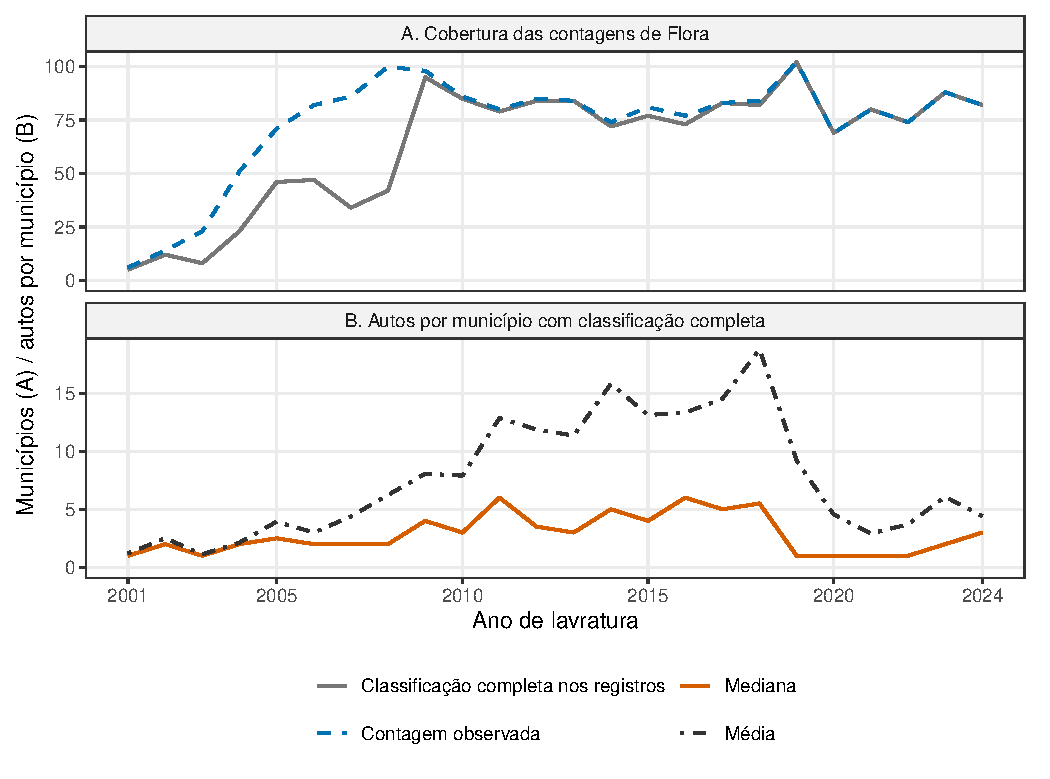
\includegraphics[width=\textwidth]{assets/fig04_ibama.pdf}
    \caption{Cobertura e distribuição das autuações do IBAMA classificadas como Flora}
    \label{fig:h1-ibama}
    \begin{minipage}{\textwidth}\footnotesize
    \centering
    Fonte: elaboração própria com registros do IBAMA e malha IBGE 2023.
    \end{minipage}
\end{figure}
\FloatBarrier

A média (cinza-escuro, traço-ponto) passou de 18,77 autos em 2018 para 4,41 em 2024; a mediana (laranja contínuo), de 5,5 para 3. O total de municípios classificados foi 82 em cada ano, sem garantia de mesma composição. A cobertura anual variou entre \HibMin{} e \HibMax{} municípios. A distância entre média e mediana evidencia contagens elevadas em parte do grupo, mas não permite ordená-lo por risco de punição.

A variação dessas contagens reúne processos com implicações distintas para os incentivos: menos autos podem refletir maior cumprimento das regras, menor detecção ou mudanças de registro, enquanto mais autuações onde há conversão podem decorrer de fiscalização direcionada às infrações. Essa possibilidade não contradiz o efeito de contenção identificado por \citeonline{AssuncaoEtAl2023}, cuja estratégia explorou limitações de detecção por nuvens no DETER. A diferença está no que cada medida e desenho permitem observar, pois os autos aqui descritos não medem efetividade, e as transições de uso da terra não distinguem conversões regulares de irregulares.

As condições institucionais também podem afetar a receita esperada ao vincular o acesso aos mercados a exigências ambientais. A possibilidade de perder compradores modifica a atratividade de produzir em áreas que descumpram os critérios de compra, como no mecanismo da Moratória da Soja examinada por \citeonline{HeilmayrEtAl2020}. Essa relação dá às vendas externas uma função na contextualização dos incentivos, distinta daquela desempenhada pelos registros de autuação.

O Código Florestal estabelece obrigações de proteção e recomposição da vegetação nos imóveis \cite{Brasil2012}, enquanto a Moratória condiciona a comercialização da soja segundo critérios do acordo no bioma Amazônia. Esses instrumentos não têm a mesma abrangência, e o bioma predominante do município não informa a obrigação de cada imóvel ou a exposição de cada lavoura. Assim, autuações, localização territorial e comércio caracterizam dimensões institucionais diferentes. Sua descrição prepara a comparação das associações entre preços e conversão sob restrições distintas, sem medir diretamente o efeito de cada política.

A Figura~\ref{fig:h1-exportacoes} dimensiona o comércio, sem medir cumprimento desses compromissos. Os painéis superiores mostram FOB em bilhões de dólares correntes; os inferiores, peso líquido em milhões de toneladas. As colunas são soja, milho e carne, com escalas verticais próprias e os mesmos produtos e critérios da Tabela~\ref{tab:h1-oferta-contexto}.

\begin{figure}[htbp]
    \centering
    % Título e fonte ficam apenas no LaTeX; o recorte preserva painéis e eixos.
    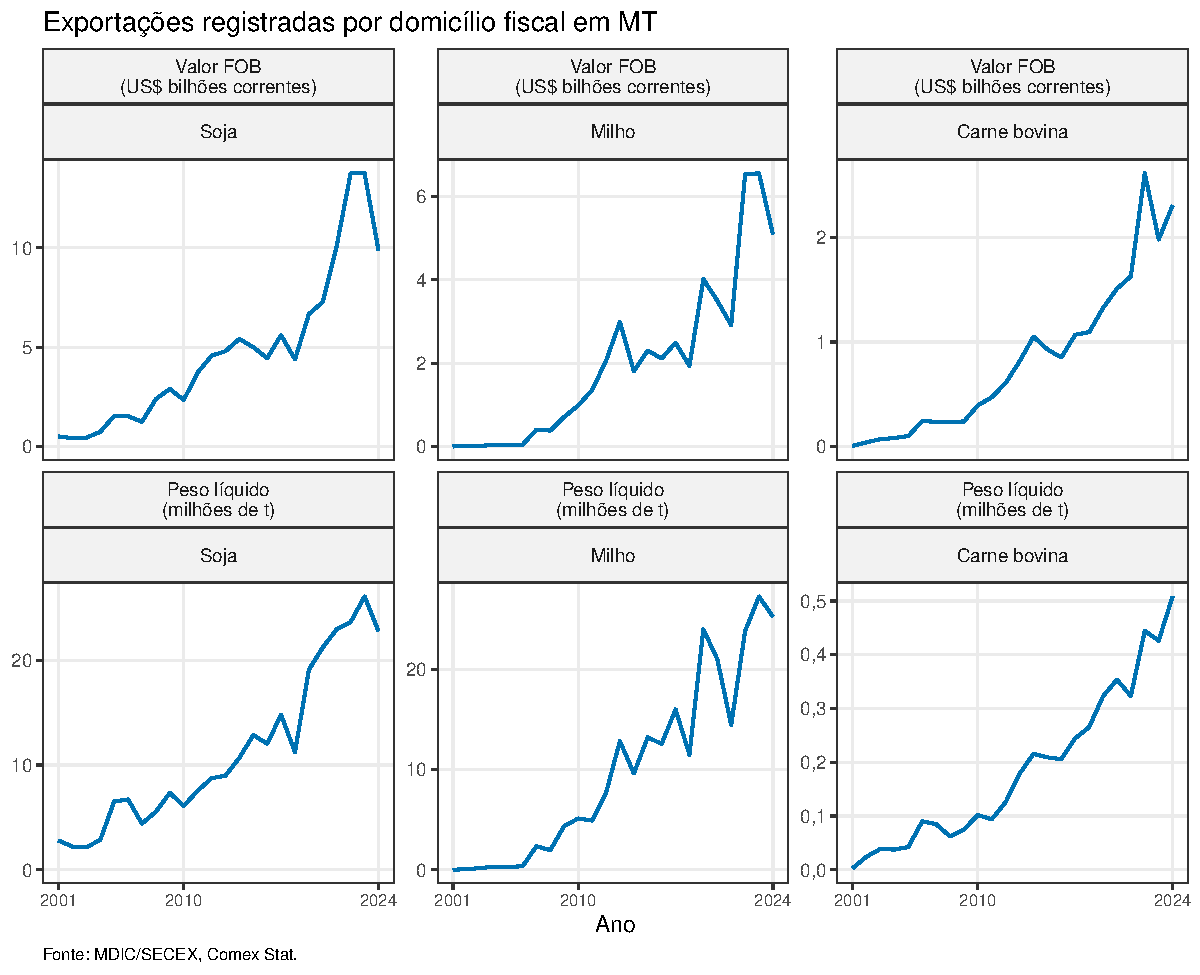
\includegraphics[width=\textwidth,trim=0 16bp 0 20bp,clip]{assets/fig09_exportacoes.pdf}
    \caption{Valor e peso líquido das exportações registradas por domicílio fiscal em Mato Grosso}
    \label{fig:h1-exportacoes}
    \begin{minipage}{\textwidth}\footnotesize
    \centering
    Fonte: elaboração própria com MDIC/SECEX, Comex Stat.
    \end{minipage}
\end{figure}
\FloatBarrier

Em 2024, foram exportados 22,79 milhões de toneladas de soja, 25,28 de milho e 0,51 de carne bovina. Essa escala comercial dimensiona oportunidades de receita nos mercados externos, enquanto as autuações descrevem uma parte da atuação administrativa sobre a produção e o uso dos recursos. O domicílio fiscal, porém, não localiza diretamente a produção ou a área convertida, e essas séries não identificam o efeito das instituições. Para compreender as condições em que os incentivos operam, é necessário observar também como atividades produtivas, vegetação e possibilidades de expansão se distribuem pelo território.

\FloatBarrier
\subsection{Heterogeneidade econômica e ambiental de Mato Grosso}
\label{descritiva-heterogeneidade}

A distribuição das atividades e da vegetação situa as alternativas de uso em contextos territoriais distintos. Onde já existem lavouras e pastagens, a expansão pode envolver reorganização produtiva, enquanto a presença de vegetação remanescente mantém a conversão entre as possibilidades de uso. Localizar esses elementos permite compreender a diversidade de trajetórias que uma média estadual reúne.

\citeonline[Fig.~6]{SimoesEtAl2020} documentaram expansão de pastagens sobretudo ao norte, no bioma Amazônia (Seção~\ref{literatura-sintese}). A Figura~\ref{fig:h1-uso-solo} retoma essa perspectiva espacial com mapas próprios de 2001 e 2024, baseados no MapBiomas e em agregação distinta. A classe denominada ``Soja e Milho'' concentra-se nas porções central e leste, e a cobertura florestal, ao norte. A comparação contextualiza a localização dos usos, sem constituir extensão direta da série daquele estudo.

\begin{figure}[htbp]
    \centering
    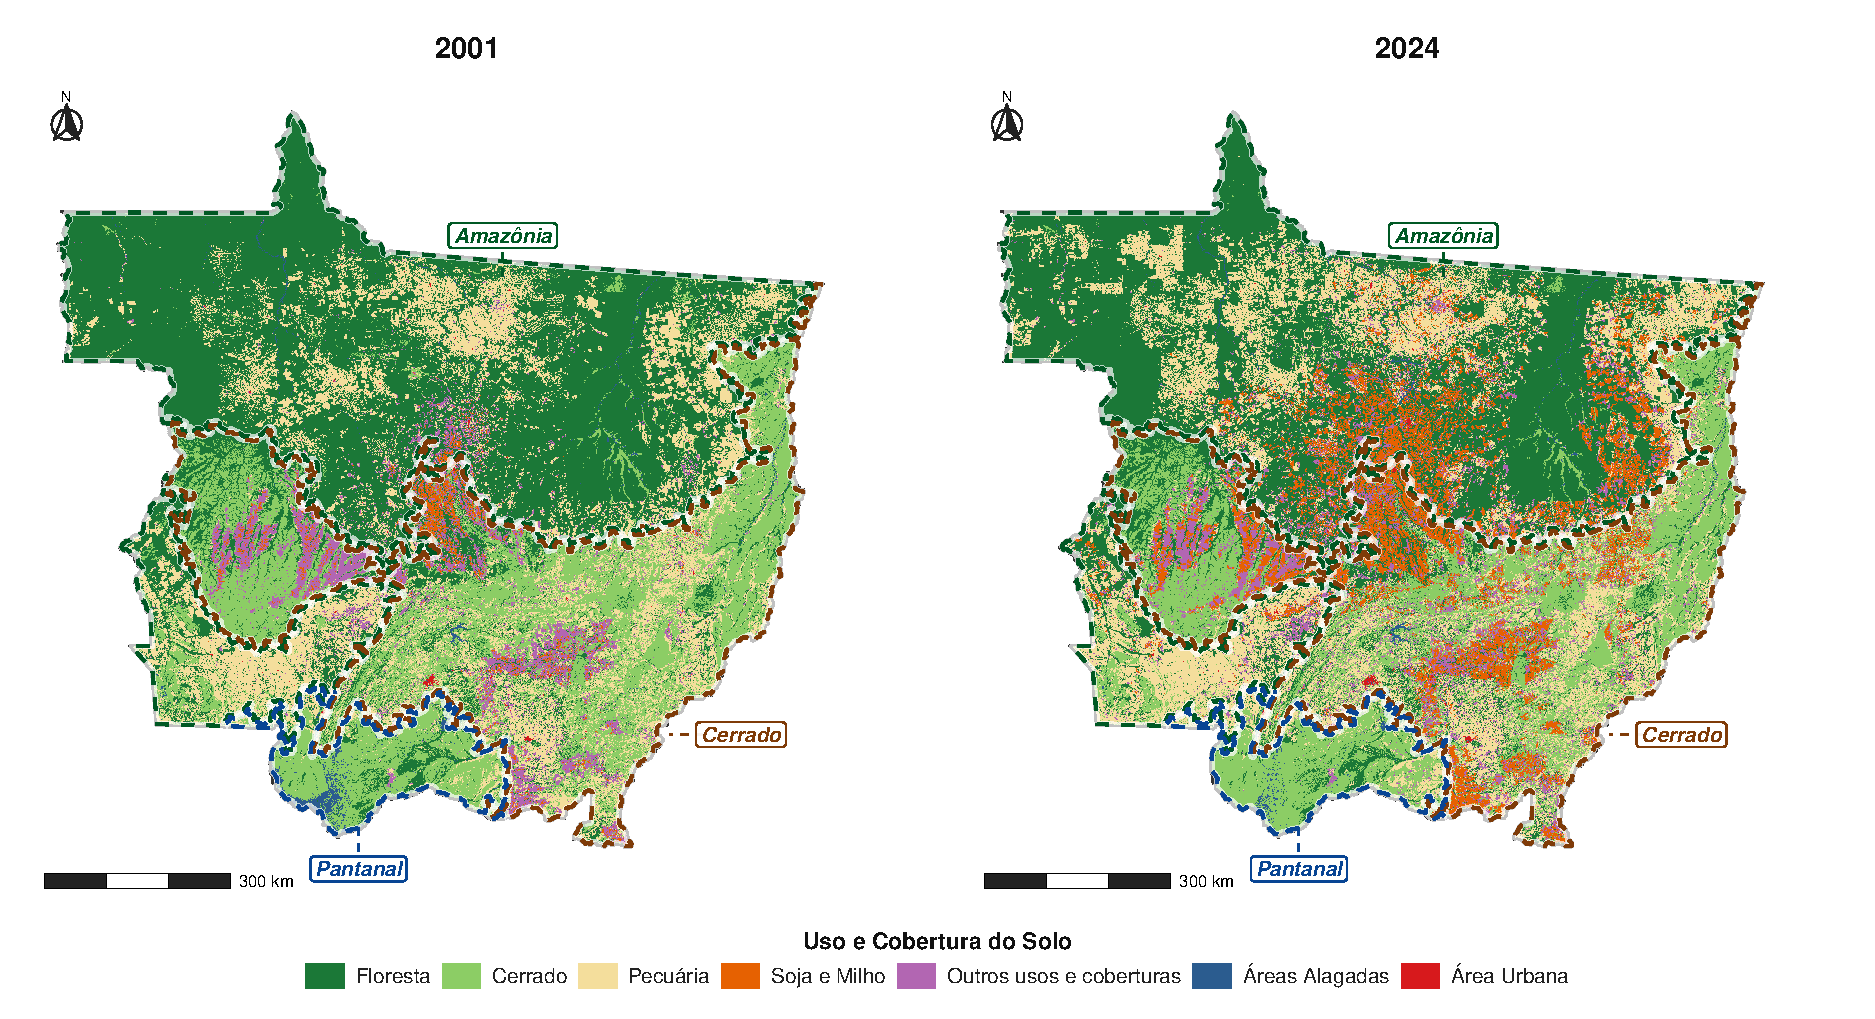
\includegraphics[width=\textwidth]{assets/fig6_uso_solo_mt_2001_2024.pdf}
    \caption{Distribuição espacial de classes agregadas de uso e cobertura do solo em Mato Grosso, 2001 e 2024}
    \label{fig:h1-uso-solo}
    \begin{minipage}{\textwidth}\footnotesize
    Fonte: elaboração própria com camadas do MapBiomas e limites do IBGE.
    \end{minipage}
\end{figure}
\FloatBarrier

Na legenda, ``Soja e Milho'' combina soja e segunda safra de grãos, não todas as áreas dessas culturas. ``Pecuária'' representa pastagens; ``Cerrado'', formações savânicas, campestres e outras nativas, não o limite do bioma. ``Áreas Alagadas'' designa corpos d'água; ``Outros usos e coberturas'' inclui vegetação secundária e classes residuais. As duas datas contextualizam usos, mas não identificam transições anuais, perda total de vegetação ou expansão líquida das lavouras.

Essa distribuição também se relaciona com restrições que variam entre lugares. A Moratória examinada por \citeonline{HeilmayrEtAl2020}, por exemplo, estabeleceu critérios específicos para o bioma Amazônia. A comparação territorial reúne, assim, condições ambientais e exposição a instrumentos de conservação, sem isolar cada uma delas.

Para comparar conversão, os municípios foram agrupados pelo bioma de maior fração de área, pela interseção da malha IBGE 2023 com biomas IBGE 2019. As frações foram preservadas: \Hmixed{} municípios são mistos, com mais de um bioma acima de $10^{-6}$ da área. Os fluxos não foram repartidos por essas frações, pois isso lhes atribuiria localização não informada pelos agregados. O grupo não localiza cada conversão dentro de um bioma nem implica regras uniformes em todo o município.

Na Tabela~\ref{tab:h1-cobertura}, pares válidos têm cobertura integral do par de mapas; municípios fixos têm conversão observada nos 24 anos. A cobertura alcança 71,6\% dos pares potenciais amazônicos, 96,4\% dos do Cerrado e 56,2\% dos pantaneiros. Apenas um dos quatro municípios de predominância pantaneira é fixo. Manter composição constante não assegura representatividade estadual, suporte equivalente entre grupos ou compatibilidade histórica de todas as fontes.

\begin{table}[htbp]
\centering
\small
\caption{Cobertura da conversão por predominância territorial, 2001--2024}\label{tab:h1-cobertura}
\begin{tabular}{lrrrrr}
\hline
Grupo & Municípios & Mistos & Pares válidos & \% da grade & Fixos \\
\hline
Amazônia & 76 & 35 & 1.306 & 71,6 & 39 \\
Cerrado & 61 & 24 & 1.412 & 96,4 & 55 \\
Pantanal & 4 & 4 & 54 & 56,2 & 1 \\
\hline
\end{tabular}
\par\smallskip\begin{minipage}{\textwidth}\footnotesize
Fonte: elaboração própria com MapBiomas 10.1 e IBGE.
\end{minipage}
\end{table}

\FloatBarrier

Na Figura~\ref{fig:h1-distribuicao}, cada ponto é a média das 24 taxas anuais municipais, com igual peso aos anos, distinta da razão de somas da Figura~\ref{M-fig:h1-conversao}. O deslocamento horizontal separa pontos; a altura indica a média temporal. Agricultura está à esquerda e pastagem, à direita.

\begin{figure}[htbp]
    \centering
    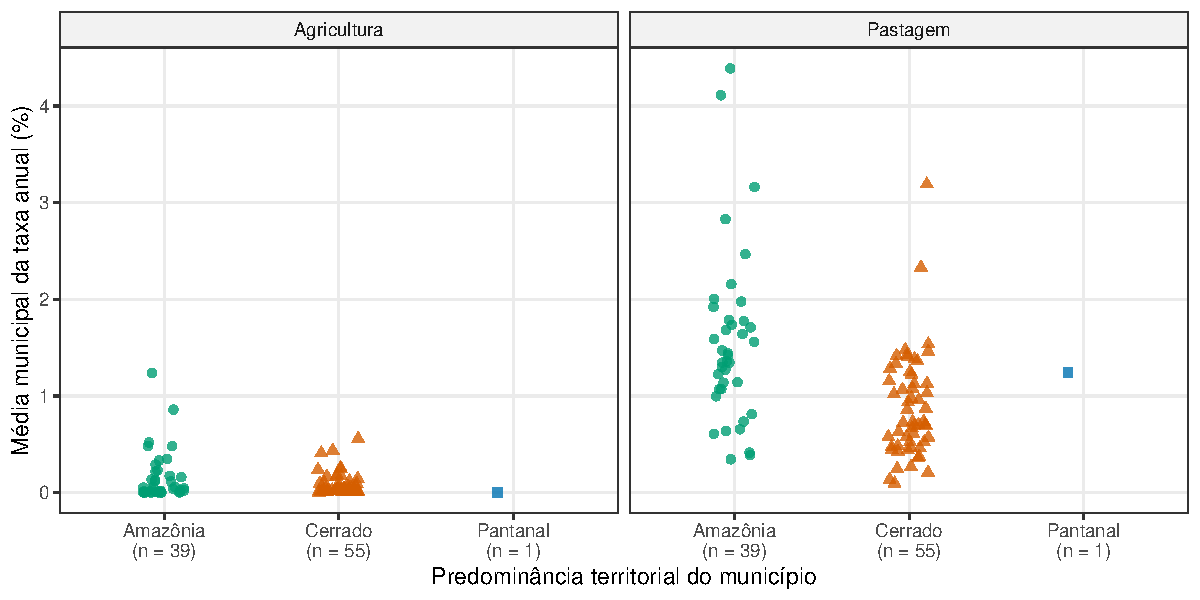
\includegraphics[width=\textwidth]{assets/fig02_distribuicao.pdf}
    \caption{Heterogeneidade das taxas médias municipais de conversão, 2001--2024}
    \label{fig:h1-distribuicao}
    \begin{minipage}{\textwidth}\footnotesize
    \centering
    Fonte: elaboração própria com MapBiomas 10.1 e IBGE.
    \end{minipage}
\end{figure}
\FloatBarrier

A dispersão das taxas entre os 39 municípios fixos de predominância amazônica e os 55 do Cerrado, sobretudo para pastagem, indica que pertencer a um mesmo bioma não esgota as diferenças territoriais, enquanto o único pantaneiro não permite caracterizar uma distribuição representativa. Na análise de \citeonline{VanWeyEtAl2013}, transportes, produção anterior e conexão com mercados estiveram associados à expansão de duas safras, situando possibilidades e custos que podem variar mesmo sob condições ambientais próximas. A capacidade potencial acrescenta uma dimensão agronômica a essas oportunidades, cuja contribuição para a dispersão observada não é identificada pelo gráfico.

Além das diferenças de acesso e de trajetória produtiva, a comparação entre municípios precisa considerar suas possibilidades agronômicas. Para representá-las, distingue-se a produção possível sob condições padronizadas do rendimento registrado pela PAM nas áreas colhidas, que incorpora manejo, insumos e seleção das parcelas cultivadas. A Tabela~\ref{tab:h1-capacidade} utiliza rendimentos potenciais do \textit{Global Agro-Ecological Zones} (GAEZ v4) \cite{FAOGAEZ2021}, em alto insumo e regime de sequeiro (sem irrigação), medidos em kg de matéria seca por hectare. Na grade original, o indicador registra o rendimento atingível na melhor classe de aptidão da célula, sendo depois agregado por município mediante média dos pixels válidos ponderada pelo cosseno da latitude para aproximar áreas. Cada um dos 141 municípios entra uma vez, com igual peso, não apenas os 95 fixos ambientais.

A climatologia selecionada é 1961--1990, mas a versão reúne bases territoriais de 2010, de modo que o indicador fixo no painel não garante anterioridade de todos os componentes às decisões de 2001--2024. A média municipal caracteriza o potencial agrícola do território, sem descrever necessariamente as parcelas nativas disponíveis ou representar capacidade pecuária. Tampouco corresponde ao rendimento anual observado, pois a unidade de matéria seca não equivale diretamente ao rendimento comercial da PAM.

\begin{table}[htbp]
\centering
\small
\caption{Rendimento potencial municipal no cenário de alto insumo e sequeiro}\label{tab:h1-capacidade}
\begin{tabular}{llrrr}
\hline
Cultura & Predominância & Municípios & Mediana & P25--P75 \\
\hline
Milho & Amazônia & 76 & 3.002 & 2.862--3.264 \\
Milho & Cerrado & 61 & 3.320 & 2.797--3.572 \\
Milho & Pantanal & 4 & 6.790 & 6.321--6.933 \\
Soja & Amazônia & 76 & 2.701 & 2.557--2.852 \\
Soja & Cerrado & 61 & 3.261 & 2.817--3.390 \\
Soja & Pantanal & 4 & 3.421 & 3.386--3.457 \\
\hline
\end{tabular}
\par\smallskip\begin{minipage}{\textwidth}\footnotesize
Fonte: elaboração própria com FAO/IIASA, GAEZ v4, e IBGE.
\end{minipage}
\end{table}

\FloatBarrier

As medianas do Cerrado e da Amazônia foram, respectivamente, 3.261 e 2.701 kg de matéria seca/ha para soja e 3.320 e 3.002 para milho. P25--P75 delimita a metade central da distribuição. As maiores medianas pantaneiras representam somente quatro municípios, todos mistos, o que impede tomá-las como caracterização homogênea desse ambiente.

As diferenças de potencial permitem considerar que, mantidos os custos e as demais condições, uma mesma alta de preço representa maior acréscimo de receita por hectare onde a terra pode produzir mais, vantagem que pode favorecer tanto o aproveitamento de áreas abertas quanto novas conversões. A tabela caracteriza essas possibilidades produtivas, enquanto a pergunta do artigo se refere a como elas modificam a associação entre preços e abertura de áreas. Como o nível isolado da capacidade é absorvido pelos efeitos fixos municipais, o contraste de H1a acompanha sua interação com a variação anual dos preços, utilizando a heterogeneidade descrita na tabela sem tomá-la como teste da hipótese. O potencial padronizado situa o que a terra pode produzir; o desempenho das safras anteriores acrescenta outra dimensão às condições sob as quais os incentivos operam.

\subsection{Perdas produtivas anteriores e condições de resposta aos preços}
\label{descritiva-perdas}

Uma safra abaixo de sua referência local pode modificar as condições de investimento mesmo onde o potencial agrícola é elevado. Para caracterizar essa diferença, a produção por hectare plantado reúne o rendimento da área colhida e a parcela da área plantada que chegou à colheita. A razão entre produção e área colhida, isoladamente, pode omitir perdas de área. Essa distinção aproxima a mensuração das hipóteses explicativas discutidas na revisão: perdas físicas podem restringir recursos ou ser seguidas de expansão, mas não medem diretamente caixa, prejuízo financeiro ou intenção de recompor a produção. Os resultados de \citeonline{AssuncaoEtAl2020Credito} sobre crédito e de \citeonline{OrdonezEtAl2025} sobre choques produtivos situam possibilidades distintas, sob condições que não são reproduzidas automaticamente pela comparação municipal de Mato Grosso.

A referência de cada safra é prevista por uma tendência linear ajustada aos dez anos anteriores do próprio município e cultura, exigindo ao menos sete observações válidas e previsão positiva. A intensidade da perda, $L$, é a parte positiva de um menos a razão entre produção por hectare plantado e essa referência. Logo, $L=0$ reúne desempenhos iguais ou superiores à referência, enquanto $L=0{,}20$ indica déficit de 20\%. O indicador D20 distingue perdas de pelo menos 20\%, como corte operacional complementar à medida contínua. Não se atribui perda zero a ausência de cultivo, informação indisponível ou histórico insuficiente. As alternativas por mediana, janelas de cinco e quinze anos, área colhida e cortes de 10\% e 30\% permitem avaliar a sensibilidade dessa mensuração, sem escolher a definição pelo resultado econométrico.

Para a conversão entre os mapas de $t-1$ e $t$, a descrição relaciona a perda da safra $t-2$ ao preço anual de $t-1$. Assim, as conversões de 2001 e 2024 são vinculadas, respectivamente, às safras de 1999 e 2022 e aos preços de 2000 e 2023. O histórico usado na previsão termina antes de cada safra. Essa ordenação evita utilizar produção posterior para definir a perda, mas não identifica a data de abertura dentro do intervalo dos mapas ou demonstra planejamento intertemporal. O milho permanece agregado por ano, sem separar primeira e segunda safras. O reinício das referências após rupturas territoriais identificadas reduz uma fonte de descontinuidade, sem equivaler à harmonização integral dos limites históricos.

Essa exigência de cultivo e histórico restringe a comparação a localidades e anos em que a perda pode ser medida. A Tabela~\ref{tab:h1b-cobertura} apresenta os pares com conversão observada e perda válida dois anos antes. A coluna de cobertura divide esses pares pelas observações de conversão disponíveis em cada bioma, e D20 conta aqueles com perda de pelo menos 20\%. Restam 1.488 pares para soja, 53,7\% dos 2.772 observados, e 2.381 para milho, 85,9\%. Na soja, a cobertura é menor na Amazônia que no Cerrado; o milho conserva proporções próximas nesses dois grupos. No Pantanal, a cobertura relativa do milho é elevada dentro de uma base ambiental já pequena: são 52 pares em três municípios. Os 28 pares de soja pertencem a apenas dois municípios, o que restringe a comparação territorial das perdas.

\begin{table}[htbp]
\centering\small\captionstyle{\centering}\normalcaption
\caption{Cobertura das perdas anteriores nas observações de conversão, 2001--2024}\label{tab:h1b-cobertura}
\begin{tabular}{llrrrr}
\hline
Cultura & Bioma & Pares & Municípios & Cobertura (\%) & D20 \\
\hline
Soja & Amazônia & 561 & 59 & 43,0 & 8 \\
Soja & Cerrado & 899 & 54 & 63,7 & 32 \\
Soja & Pantanal & 28 & 2 & 51,9 & 2 \\
Soja & MT & 1.488 & 115 & 53,7 & 42 \\
Milho & Amazônia & 1.117 & 74 & 85,5 & 122 \\
Milho & Cerrado & 1.212 & 60 & 85,8 & 153 \\
Milho & Pantanal & 52 & 3 & 96,3 & 8 \\
Milho & MT & 2.381 & 137 & 85,9 & 283 \\
\hline
\end{tabular}
\par\smallskip\begin{minipage}{\textwidth}\footnotesize\centering
Fonte: elaboração própria com IBGE/PAM e MapBiomas 10.1.
\end{minipage}
\end{table}

\FloatBarrier

As contagens de elegibilidade antecedem a remoção de grupos unitários de efeitos fixos: a estimação utiliza 1.459 pares de soja e 2.376 de milho. A diferença entre disponibilidade e amostra efetiva é explicitada na Seção~\ref{estrategia-amostra}, preservando a função descritiva das tabelas e gráficos desta seção.

A seleção não modifica apenas o número de observações. Na Tabela~\ref{M-tab:h1b-composicao}, cada célula apresenta média e, entre parênteses, mediana, com igual peso aos pares município--ano. A coluna observada reúne os 2.772 pares de conversão; soja e milho são seus subconjuntos com perda anterior válida, que se sobrepõem. As taxas usam o estoque nativo inicial como denominador municipal, e os potenciais fixos reaparecem a cada ano observado, diferindo da distribuição com um registro por município da Tabela~\ref{tab:h1-capacidade}. A conversão agrícola média passa de 0,112\% no conjunto observado para 0,106\% na amostra de soja e 0,085\% na de milho. As distâncias entre médias e medianas mostram que a média reúne taxas muito diferentes. Por isso, uma mudança de estimativa após incluir perdas pode refletir tanto a especificação quanto a composição amostral, exigindo comparar H1a nas mesmas observações utilizadas para H1b.



A anomalia anual de chuva na tabela é a diferença entre a precipitação em $t$ e a média municipal de 1981--2000, em milímetros. Ela caracteriza uma condição que varia no tempo e participa da estratégia empírica, sem medir diretamente o clima da safra $t-2$. A chuva pode afetar o desempenho agrícola e a própria vegetação, de modo que sua relação com perdas não basta para torná-la instrumento válido. Essa distinção importa para interpretar H1b: uma associação atribuída às perdas pode reunir efeitos climáticos diretos, mudanças de manejo e outros choques locais, além dos mecanismos financeiros discutidos na literatura.

A Figura~\ref{M-fig:h1b-perdas} mostra por que a referência produtiva e a cobertura precisam acompanhar a leitura das perdas. As colunas correspondem a soja e milho, e o eixo horizontal registra a safra anterior. Nos painéis superiores, a produção total é dividida pela área plantada ou colhida total dos mesmos municípios elegíveis; a referência é a média das previsões locais ponderada pela área plantada corrente. Nos painéis intermediários, a perda média dá igual peso aos municípios e a frequência divide os casos D20 pelo número elegível, apresentado nas barras inferiores. A média das perdas é calculada a partir das medidas municipais, e não da distância entre as curvas agregadas superiores. Essas duas medidas não representam a fração da produção estadual perdida. A composição varia entre safras, de modo que as curvas não descrevem uma amostra municipal fixa.



A proximidade das razões por área plantada e colhida em grande parte das safras não elimina diferenças locais, pois as somas dão maior peso às áreas extensas. Na amostra de milho de 1999, as razões foram 2,33 e 2,79 t/ha, respectivamente, enquanto em 2016 foram 4,08 e 4,26 t/ha. Nessa última safra, a referência ponderada foi 6,22 t/ha, a perda municipal média atingiu 26,7\% e 58,7\% dos 109 municípios elegíveis registraram D20. O contraste reúne redução do desempenho em áreas colhidas e não colheita de parte da área plantada, sem identificar sua causa. Na soja, a perda média foi 13,5\% em 2004 e 11,3\% em 2016, com 40 e 76 municípios. A variação de cobertura impede interpretar a diferença entre essas médias como mudança do risco em um grupo constante.

As perdas também são distribuídas de forma desigual entre os níveis de preço. A Figura~\ref{fig:h1b-contrastes} aproxima as variáveis da pergunta do artigo: apresenta médias das taxas municipais de conversão agrícola, com igual peso aos pares município--ano, por quatro grupos de anos ordenados pelo preço real de cada cultura no ano anterior. Cada grupo contém seis dos 24 anos de preços, não necessariamente consecutivos. À esquerda, os municípios são separados pela mediana do potencial entre os 141 territórios, fixa no tempo. À direita, a classificação distingue perda zero, perda positiva inferior a 20\% e D20. Soja está acima e milho abaixo. Os quadros inferiores informam o número de pares em cada célula; nem todas elas contêm observações dos seis anos. Cada cultura utiliza a mesma amostra candidata nos dois painéis, sem ajuste por efeitos fixos ou controles.

\begin{figure}[htbp]
    \centering
    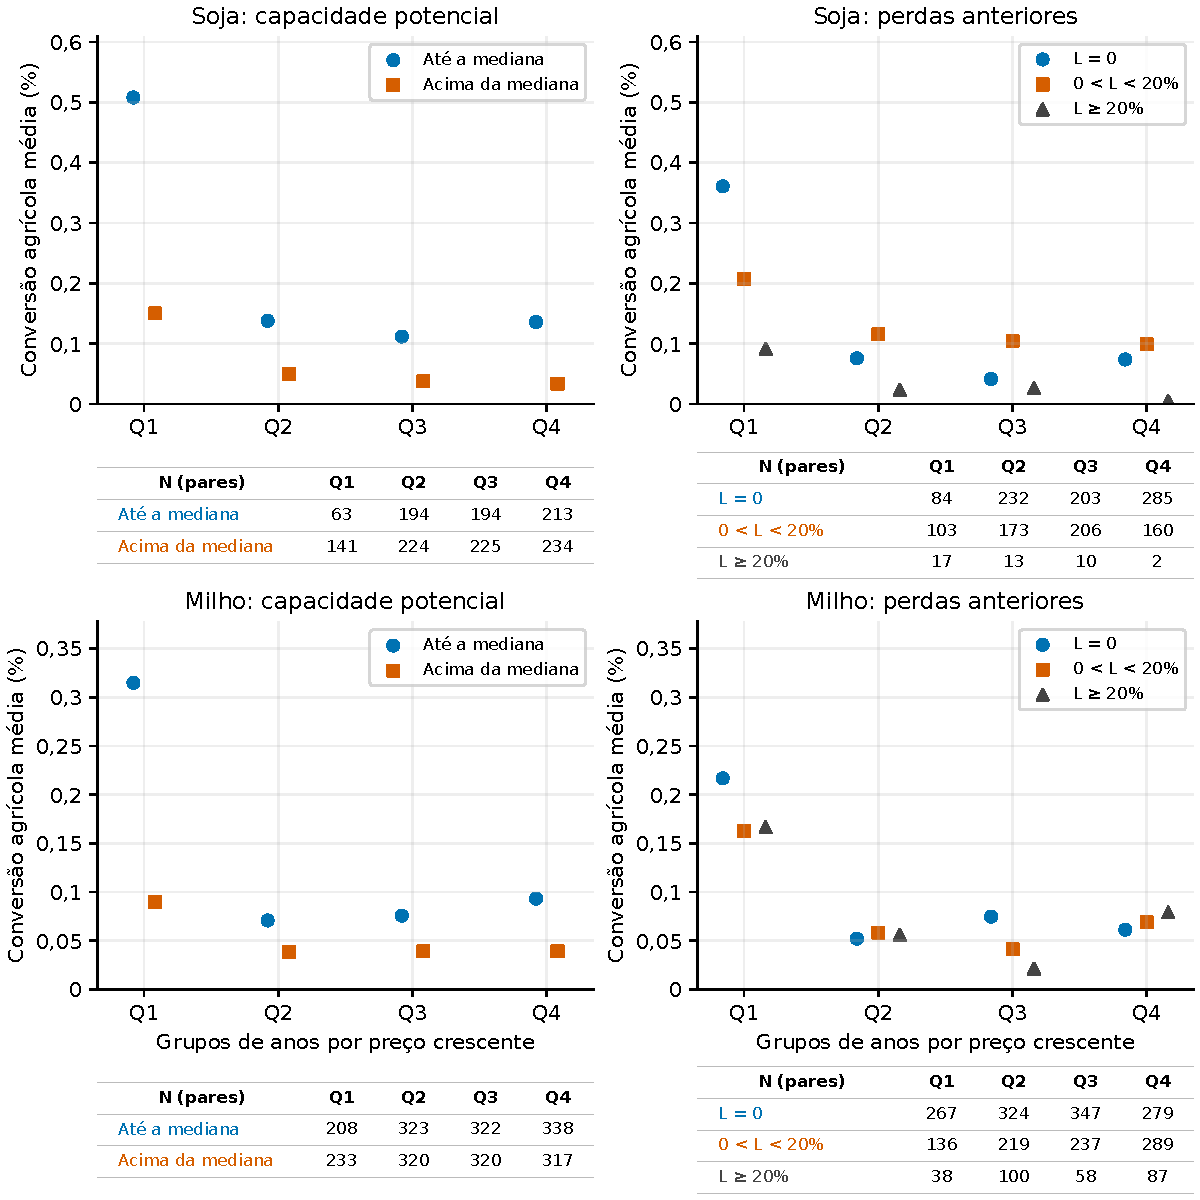
\includegraphics[width=\textwidth]{assets/fig11_precos_modificadores_etapa5.pdf}
    \caption{Conversão agrícola por grupos de preços, capacidade potencial e perdas anteriores}
    \label{fig:h1b-contrastes}
    \begin{minipage}{\textwidth}\footnotesize\centering
    Fonte: elaboração própria com MapBiomas, IBGE/PAM, GAEZ v4, Banco Mundial e CPI-U BLS/FRED.
    \end{minipage}
\end{figure}
\FloatBarrier

As médias brutas não exibem uma ordenação positiva uniforme entre preço e conversão. No primeiro grupo de preços, a conversão média é maior entre municípios de menor potencial nas duas culturas, e as diferenças mudam nos demais grupos. Esse grupo concentra cotações do início da série: 2000--2003, 2005 e 2006 para soja, e 2000--2005 para milho. A comparação por preço reúne, assim, diferenças de período e de localidades, o que torna pertinentes os efeitos de tempo e as tendências na análise econométrica. O padrão bruto não constitui rejeição de H1a, cuja proposição se refere à diferença da associação condicionada às demais características relevantes.

Para H1b, a escassez de algumas combinações é parte do resultado descritivo: a soja tem apenas dois pares com D20 no grupo de preços mais altos, distribuídos em dois anos. No milho, a média desse grupo supera a do grupo imediatamente anterior, mas a comparação reúne outras mudanças de composição e de contexto. Os pontos não identificam restrição de recursos, recomposição da produção ou efeito da quebra; tornam visíveis os contrastes e o suporte examinados na estimação. Esses mecanismos permanecem hipóteses explicativas a confrontar com evidências próprias, e o sinal da modificação proposta em H1b continua indeterminado.

\subsection{Síntese das evidências e implicações para a análise econométrica}
\label{descritiva-sintese}

O crescimento da produção e do comércio coexistiu com taxas de conversão menores nos extremos do período e predomínio da pastagem na amostra fixa. A descrição também mostrou que a composição da expansão produtiva, as taxas municipais, a capacidade potencial e as perdas anteriores diferem entre culturas e territórios. Esses fatos situam a questão da resposta aos incentivos: a trajetória comum dos preços pode ser acompanhada de associações distintas com a conversão conforme as possibilidades agrícolas de cada município e seu desempenho anterior. O papel da base natural e das condições locais aparece nessas diferenças; a ordenação entre safra, preço e conversão incorpora a dimensão temporal sem medir expectativas individuais.

A comparação econométrica precisa distinguir essas associações da influência de outros fatores que também mudam ao longo do tempo. H1a requer comparar a associação preço--conversão conforme a capacidade potencial; H1b, examinar sua modificação pela perda anterior, incluindo a interação entre preço e perda, além do termo da própria perda. A redução da amostra, a concentração de ocorrências e as diferenças entre médias brutas delimitam esses contrastes e justificam as comparações em amostras comuns. Agricultura permanece como destino principal, e pastagem permite examinar se o padrão se restringe à abertura agrícola. Na dimensão institucional complementar, autuações e embargos têm limites de cobertura que impedem tratá-los como exposição legal ou comercial. A Seção~\ref{sec:estrategia} distingue esses registros da fração amazônica usada para caracterizar o alcance potencial da Moratória e da cobertura florestal de 2000 usada na comparação em torno da reforma de 2012. A segunda medida reúne as classes Formação Florestal e Floresta Alagável do MapBiomas, sem representar obrigação de Reserva Legal ou passivo por imóvel. A discussão dos resultados confronta os coeficientes e sua precisão com essas condições, preservando resultados contrários às hipóteses e sem atribuir às perdas um mecanismo único.

\endgroup


\section{Construção das variáveis, calendário e núcleo empírico}
\label{text:s3}
\label{sec:estrategia}

A comparação descritiva mostrou que o crescimento da produção de grãos coexistiu com taxas de conversão menores nos extremos do período e com predomínio da pastagem entre as áreas abertas na amostra fixa. Também evidenciou diferenças na capacidade potencial, nas perdas anteriores e no histórico disponível para medi-las. Essas trajetórias não revelam, por si, como a associação entre preços e conversão varia com as condições produtivas. Para examinar H1a e H1b, a estratégia combina a variação anual das cotações com diferenças municipais de capacidade e de desempenho anterior, considerando características permanentes e mudanças comuns aos grupos de bioma predominante.

\subsection{Construção da perda, calendário e amostra de estimação}
\label{estrategia-amostra}

A análise utiliza a grade anual dos 141 municípios de Mato Grosso na malha do IBGE de 2023, entre 2001 e 2024, que perfaz 3.384 pares município--ano potenciais. A restrição aos pares com cobertura completa das transições do MapBiomas Coleção 10.1 exclui 612 observações e preserva 2.772 pares em 137 municípios \cite{MapBiomas2026}. Os valores preenchidos na base auxiliar não são tratados como conversões observadas. Esse conjunto ainda difere das amostras efetivas, pois o histórico produtivo necessário às perdas e os grupos unitários de efeitos fixos acrescentam exclusões.

A perda compara o desempenho realizado de cada cultura com uma referência construída exclusivamente com seu passado local. Para município $i$, cultura $c\in\{\mathrm{soja},\mathrm{milho}\}$ e safra $s$, define-se o desempenho $a_{ic,s}=Q_{ic,s}/AP_{ic,s}$, em toneladas por hectare plantado. $Q$ é a produção e $AP$ a área plantada publicada na PAM \cite{IBGEPAM2026}. A referência $\widehat a_{ic,s|s-1}$ é a previsão de uma tendência linear local ajustada às observações válidas entre $s-10$ e $s-1$, com pelo menos sete anos e previsão positiva. A intensidade da perda é
\begin{equation}
L_{ic,s}=\max\left\{0,\,1-\frac{a_{ic,s}}{\widehat a_{ic,s|s-1}}\right\}.
\label{eq:perda-produtiva}
\end{equation}
Assim, $L=0$ reúne desempenhos iguais ou superiores à referência, enquanto $L=0{,}20$ indica déficit de 20\%. O indicador complementar $D20_{ic,s}=\mathbb{I}[L_{ic,s}\geq0{,}20]$ descreve a ocorrência segundo um limiar operacional. Ausência de cultivo, informação indisponível e histórico insuficiente não recebem perda zero. A construção emprega os registros originais da PAM, sem usar interpolação para identificar safras, e reinicia a referência após rupturas territoriais identificadas. Essa precaução não assegura harmonização integral dos limites históricos.

A razão por área plantada reúne rendimento colhido e proporção da área que chegou à colheita, como discutido na Seção~\ref{descritiva-perdas}. Ela incorpora também mudanças de manejo, composição das parcelas e mensuração. A tendência móvel permite acompanhar parte da evolução produtiva, mas uma previsão baseada em poucos anos pode ser instável. A medida não isola choques climáticos ou biológicos e não corresponde diretamente a prejuízo financeiro. O rendimento realizado usado para construir $L$ permanece distinto do potencial agronômico padronizado empregado em H1a.

Para a conversão registrada entre os mapas de $t-1$ e $t$, utiliza-se a perda da safra $t-2$ e o preço médio real de $t-1$. Em 2001, a perda corresponde a 1999 e sua referência usa 1989--1998; em 2024, a perda corresponde a 2022 e o preço, a 2023. A safra antecede o ano de preço, mas os mapas anuais não localizam a abertura dentro do intervalo nem permitem recuperar a informação de cada produtor no momento da decisão. O milho permanece agregado por ano, sem separar primeira e segunda safras.

Com perda válida em $t-2$, são elegíveis 1.488 pares de soja em 115 municípios e 2.381 de milho em 137, conforme a descritiva. A remoção recursiva de grupos com uma única observação nos efeitos fixos retira, respectivamente, 29 e cinco pares. As amostras efetivas são, portanto, 1.459 pares em 106 municípios para soja e 2.376 em 134 para milho, ambas cobrindo 2001--2024. Não há exclusão adicional por falta de chuva, preço ou capacidade nessas amostras. No Pantanal, restam oito pares de soja em dois municípios e cinquenta de milho em três, suporte insuficiente para uma análise autônoma precisa do bioma.

Essa seleção favorece localidades e anos com cultivo e histórico observável. Para separar mudança de composição de mudança de fórmula, estima-se primeiro o modelo sem perdas no conjunto de conversão observada, com 2.767 pares após os efeitos fixos, e depois nas mesmas chaves efetivas utilizadas para H1b. As diferenças entre essas estimativas são comparações descritivas entre modelos, não efeitos causais da seleção ou das perdas.

\subsection{Especificação de referência e contrastes de H1a e H1b}
\label{estrategia-especificacao}

O modelo de referência preserva a exposição preço--capacidade e acrescenta a perda anterior e sua interação com o preço. Para cada cultura, estima-se por mínimos quadrados, sem ponderação,
\begin{equation}
\begin{aligned}
Y_{it}^{\mathrm{agr}}={}&\beta_c p_{ct}Z_{ic}+\theta_c L_{ic,t-2}
 +\delta_c p_{ct}L_{ic,t-2}\\
&+\gamma_c Z_{ic}\tau_t+\eta_c R_{it}
 +\alpha_i+\lambda_{b(i),t}+\varepsilon_{it}.
\end{aligned}
\label{eq:modelo-principal}
\end{equation}
A variável dependente $Y_{it}^{\mathrm{agr}}$ é cem vezes a razão entre a área de vegetação nativa convertida para agricultura e o estoque nativo disponível no início do intervalo, em pontos percentuais. Trata-se de transição bruta, não de diferença líquida entre estoques. Agricultura designa o destino imediato, sem identificar conversão especificamente para soja ou milho.

O termo $p_{ct}$ é o logaritmo do preço real internacional da cultura no ano $t-1$, centrado na média dos 24 anos. As médias anuais provêm da \textit{Pink Sheet}, com deflação mensal pelo CPI-U para dólares de 2024 \cite{WorldBank2026,BLSCPI2026}. O potencial $Z_{ic}$ corresponde ao rendimento municipal do GAEZ v4 em sequeiro e alto nível de insumos \cite{FAOGAEZ2021}, padronizado pela média e pelo desvio-padrão populacional dos 141 municípios. Essas normalizações permanecem fixas nas comparações de amostra. O potencial representa possibilidades sob um cenário tecnológico, não o rendimento observado ou a tecnologia efetivamente empregada nas parcelas convertidas.

Os efeitos municipais $\alpha_i$ absorvem características invariantes, incluindo $Z_{ic}$ isolado. Os efeitos de bioma predominante por ano $\lambda_{b(i),t}$ absorvem mudanças anuais comuns a Amazônia, Cerrado e Pantanal, incluindo $p_{ct}$ isolado. Portanto, os coeficientes das interações identificam diferenças na associação com o preço, não sua resposta média comum. O termo $Z_{ic}\tau_t$, com $\tau_t=(t-2001)/10$, admite trajetórias lineares distintas segundo a capacidade. $R_{it}$ é a anomalia anual de chuva em $t$, em centenas de milímetros, em relação a 1981--2000. A referência conserva esse controle para permitir a comparação com os modelos anteriores; as alternativas climáticas acrescentam informações da safra e do intervalo de conversão.

Na Equação~\eqref{eq:modelo-principal}, $\beta_c$ corresponde a H1a: um valor positivo indica associação preço--conversão mais positiva por um desvio-padrão adicional de capacidade, mantida a perda. $\delta_c$ corresponde a H1b: mede quanto essa associação muda por unidade adicional de perda, mantida a capacidade. Seu teste é bilateral, pois não se impõe sinal. Já $\theta_c$ descreve a associação da perda no preço geométrico médio usado na centragem e, isoladamente, não testa H1b. Os termos constitutivos $L$ e $pL$ estão presentes; os níveis de $p$ e $Z$ são absorvidos pelos efeitos fixos.

Para apresentar magnitudes, considera-se um aumento de 10\% no preço. A diferença associada a 1 DP adicional de capacidade é $\beta_c\ln(1{,}10)$; a diferença associada a dez pontos percentuais de perda é $\delta_c\ln(1{,}10)\times0{,}10$. Ambas estão em pontos percentuais da conversão bruta. Esses contrastes não recuperam o componente comum do preço nem constituem previsões de hectares municipais.

Denomina-se A o modelo que omite $L$ e $pL$, estimado na amostra original e na amostra comum; B é a Equação~\eqref{eq:modelo-principal}. A versão D substitui $L$ por D20 e $pL$ por $pD20$, mantendo as chaves de B. As regressões por cultura facilitam a leitura, mas não isolam incentivos independentes: a correlação entre os log-preços anuais de soja e milho é 0,948. A extensão conjunta inclui as duas exposições preço--capacidade, ambas as perdas e interações preço--perda, as duas tendências por capacidade e a chuva. Sua amostra comum tem 1.450 pares em 105 municípios, e os modelos individuais são reapresentados nessa mesma interseção.



\section{Sensibilidades, inferência e condicionantes}
\label{text:s4}
\subsection{Estabilidade da mensuração, do tempo e da inferência}
\label{estrategia-inferencia}

As alternativas de perda verificam quanto a comparação depende da referência e do calendário. São examinadas mediana móvel, tendência com cinco anos e mínimo de quatro observações, tendência com quinze anos e mínimo de onze, desempenho por hectare colhido, desvio assinado e ocorrências com limiares de 10\% e 30\%. A perda em $t-1$ aproxima a colheita do intervalo de conversão, mas aumenta a sobreposição temporal. Nas alternativas que mudam a cobertura, apresentam-se a amostra própria e a interseção com a referência, reestimando B nessa interseção antes de trocar a medida.

O clima pode afetar a perda e a vegetação diretamente, de modo que chuva não é tratada como instrumento. As sensibilidades utilizam anomalias do CHIRPS no ciclo agrícola e nas parcelas sazonais do ano de conversão, além da anomalia anual da referência. Também são examinados efeitos fixos de município e ano, exclusão do Pantanal e degraus por capacidade a partir de 2006 e 2012. A janela 2006--2024 verifica a dependência dos anos iniciais. Esses exercícios não acrescentam automaticamente produção, renda ou crédito posteriores à perda, que podem representar consequências dela e alterar o contraste.

A decomposição temporal permite que as associações variem entre 2001--2005, 2006--2011 e 2012--2024. Com indicadores $D_t^{(r)}$ para os três regimes, a especificação é
\begin{equation}
\begin{aligned}
Y_{it}^{\mathrm{agr}}={}&\sum_{r=1}^{3}D_t^{(r)}\left[
\beta_{c,r}p_{ct}Z_{ic}+\theta_{c,r}L_{ic,t-2}
+\delta_{c,r}p_{ct}L_{ic,t-2}\right]\\
&+\gamma_c Z_{ic}\tau_t+\zeta_{c,1}Z_{ic}\mathbb{I}[t\geq2006]
+\zeta_{c,2}Z_{ic}\mathbb{I}[t\geq2012]\\
&+\eta_cR_{it}+\alpha_i+\lambda_{b(i),t}+\varepsilon_{it}.
\end{aligned}
\label{eq:modelo-regimes}
\end{equation}
Mantêm-se a tendência e a centragem dos preços nos 24 anos. Os testes conjuntos examinam $\delta_{c,1}=\delta_{c,2}=\delta_{c,3}=0$ e a igualdade desses três coeficientes. As janelas iniciais contêm apenas cinco e seis preços anuais. Seus marcos organizam heterogeneidade temporal e não identificam efeitos de políticas coincidentes.

O nível do preço real, sua variação e o preço relativo não são medidas equivalentes. Uma sensibilidade substitui $p$ pela diferença anual do log-preço; outra usa o log-preço em $t+1$, em amostra comum com a referência. Nesta última, o preço futuro substitui o defasado nas interações, em vez de ser acrescentado a elas. A associação com informação posterior é um diagnóstico de persistência e choques comuns, sem distinguir essas explicações de expectativas ou demonstrar planejamento intertemporal.

A inferência compara agrupamento por município, duplo agrupamento por município e ano e HAC de Newey--West com duas defasagens e pesos Bartlett sobre os escores anuais da regressão residualizada pelo procedimento de Frisch--Waugh--Lovell. Os três procedimentos preservam coeficientes, controles e amostra. Os graus de liberdade das distribuições t são $G-1$, $\min(G,T)-1$ e $T-1$, respectivamente, com $G$ municípios e $T$ anos efetivos. São reportados intervalos bilaterais individuais de 95\%. Matrizes de cluster duplo que exigiram correção de autovalores negativos são identificadas; o reparo numérico não resolve suporte escasso ou dependência mal representada.

Como há somente 24 anos de preços, a multiplicação de municípios não produz o mesmo número de choques independentes. No núcleo, avaliam-se ainda agrupamento por ano, por microrregião e por microrregião+ano, bandas HAC alternativas e \textit{bootstrap wild} restrito por ano, com 999 réplicas. Essas comparações consideram formas diferentes de dependência espacial e temporal, cuja relevância é discutida por \citeonline{Conley1999}, sem garantir que todo padrão de correlação esteja coberto. A influência é examinada pela retirada de um par, município ou ano por vez, sem substituir a amostra em função do sinal. Perturbações da referência histórica, com 499 réplicas por cultura, avaliam sensibilidade à perda construída; seus quantis são condicionais e não intervalos que incorporem toda a incerteza de dados, seleção e estimação.

Os p-valores brutos são acompanhados de ajustes de Holm nas famílias registradas. No núcleo, agrupam-se as duas culturas para cada hipótese em B, mantendo D20 como comparação sem ajuste; nas sensibilidades, dezesseis contrastes H1b por cultura e procedimento. Regimes, destinos, tripla, preço relativo, culturas conjuntas e instituições têm famílias próprias, explicitadas junto às tabelas. Os cenários condicionais recebem intervalos individuais. A organização foi registrada antes das respectivas baterias, com conhecimento dos resultados anteriores, e não constitui pré-registro externo.

\subsection{Destinos, heterogeneidade adicional e condicionantes institucionais}
\label{estrategia-logistica-instituicoes}

A comparação com pastagem examina se o gradiente se restringe à abertura imediata para agricultura, mantendo capacidade e preços das culturas. Reestima-se B com $Y_{it}^{\mathrm{past}}$, sobre as mesmas chaves e o mesmo estoque nativo inicial. A regressão de $Y_{it}^{\mathrm{agr}}-Y_{it}^{\mathrm{past}}$ permite testar as diferenças entre os gradientes e incorpora a covariância entre os destinos. Significância em um destino e ausência dela no outro não bastam para concluir diferença. O potencial agrícola não representa produtividade pecuária, e os coeficientes não localizam deslocamento entre usos \cite{MacedoEtAl2012,JungEtAl2022}.

A extensão tripla acrescenta $Z_{ic}L_{ic,t-2}$ e $p_{ct}Z_{ic}L_{ic,t-2}$ à Equação~\eqref{eq:modelo-principal}. Se o coeficiente deste último termo é $\kappa_c$, o modificador de H1b é $\delta_c+\kappa_c Z_{ic}$ e o gradiente H1a é $\beta_c+\kappa_c L_{ic,t-2}$. Testam-se conjuntamente $(\delta_c,\kappa_c)=0$, $(\beta_c,\kappa_c)=0$ e, separadamente, $\kappa_c=0$. Os gradientes são apresentados em quantis observados, com a covariância integral. A tripla é uma extensão; H1b não depende de sua inclusão.

O preço relativo à carne é $\ln[P_{c,t-1}/(1000P_{b,t-1})]$, centrado nos 24 anos, convertendo a carne de dólares por quilograma para dólares por tonelada. Essa razão contextualiza alternativas entre atividades, como na comparação de \citeonline{Braganca2018}, sem medir receita líquida. Um modelo irrestrito acrescenta separadamente preço da carne×capacidade e preço da carne×perda aos termos da cultura e testa as duas restrições de coeficientes opostos impostas pela razão. A capacidade continua sendo a de soja ou milho.

As exposições institucionais exigem uma distinção adicional. Para a Moratória, $q_i^M$ é a fração municipal no bioma Amazônia, combinada com o período desde 2007 e, alternativamente, desde 2006. O acordo foi anunciado em julho de 2006, e a referência de desmatamento passou de julho de 2006 para julho de 2008 por decisão de dezembro de 2014 \cite{GTS2015Moratoria}. O indicador temporal representa alcance potencial após o anúncio, não um protocolo uniforme de monitoramento ou cumprimento por produtor. No milho, a interação se refere ao território alcançado pelo pacto da soja, não a uma proibição comercial desse produto.

Para o Código Florestal, as obrigações dependem de características e da história dos imóveis \cite{Brasil2012,SticklerEtAl2013}. Não há painel validado de imóveis, APP, Reserva Legal e passivos que permita mensurar essa exposição jurídica. Por isso, a comparação em torno de 2012 utiliza $q_i^F$, proporção municipal de formação florestal e floresta alagável do MapBiomas em 2000, e períodos desde 2013 e, alternativamente, 2012. Trata-se de heterogeneidade geográfica pela cobertura florestal inicial, que também reflete uso anterior da terra. Ela não mede obrigação legal, desmatamento irregular ou efeito da reforma. Não se atribuem percentuais de Reserva Legal aos biomas municipais.

Cada exposição é examinada separadamente, para H1a e H1b, com todos os termos inferiores identificáveis das interações com o período. As fórmulas e os resultados estão no Texto~\ref{text:s5}. A correlação entre as duas exposições municipais é 0,715; separá-las em regressões não identifica efeitos próprios das políticas. As frações não localizam os pixels convertidos, e os quartis marginais usados nos cenários não garantem igual composição pré e pós ou suporte em todas as combinações de capacidade e perda.

As autuações descritas no Texto~\ref{text:s2} permanecem indicadores de atuação administrativa. Nos embargos, a conferência espacial encontrou 11.423 termos localizados entre os 11.513 com coordenadas no retângulo de seleção, dos quais 6.819 sem área informada. Ausências de área não foram convertidas em zero. Sem reconstrução de situação vigente em cada ano e sobreposições, não se incorporou uma medida de área embargada à nova análise. O status observado pode refletir alterações posteriores, e a fiscalização pode responder às próprias infrações \cite{Sousa2016,AssuncaoEtAl2023}. Custos e logística igualmente permanecem condicionantes econômicos relevantes, sem que as proxies anteriores sejam transportadas automaticamente para os modelos com perdas.

\subsection{Alcance da interpretação}
\label{estrategia-limites}

O desenho guarda relação com exposições interagidas e preços ponderados pela aptidão \cite{GoldsmithPinkhamEtAl2020,BermanEtAl2023}, mas essa semelhança não estabelece identificação causal. O GAEZ é fixo no painel e incorpora informações territoriais de 2010, podendo se correlacionar com atributos que seguem trajetórias próprias. Mato Grosso participa da oferta mundial de grãos; preços internacionais não são necessariamente independentes dos choques de oferta locais. A perda municipal também incorpora manejo e seleção das áreas, além do clima, cujos efeitos diretos sobre a vegetação podem permanecer nos resíduos.

Os efeitos fixos, tendências e controles delimitam associações condicionais, sem eliminar toda simultaneidade ou variável omitida. A escala municipal não identifica decisões individuais, restrição financeira, recomposição intencional de produção ou expectativas. A base natural, as condições locais e a sequência temporal fundamentam a pergunta e orientam os contrastes, mas não se tornam mecanismos demonstrados pela presença de uma interação ou defasagem. Esse alcance orienta a discussão dos resultados, inclusive quando o coeficiente tem o sinal previsto ou apresenta precisão em uma das inferências.


\section{Resultados complementares e antecedentes}
\label{text:s5}
\label{ap:complementos}
\subsection{Ocorrência, mensuração e amostras comuns}

A Tabela~\ref{tab:h1-ocorrencia-etapa9} apresenta a versão D20, que substitui a intensidade pela ocorrência de déficit de pelo menos 20\%. A diferença entre os grupos com e sem ocorrência é medida por $pD20$, mantidos capacidade, tendência, chuva e efeitos fixos. As amostras são as de B: 1.459 pares de soja e 2.376 de milho. Os intervalos são individuais; D20 é complementar e não integra o ajuste das duas culturas para a intensidade contínua. Na família principal de H1a, ajustam-se os dois coeficientes $pZ$ de B; na de H1b, os dois coeficientes $pL$ de B.

% Gerado por etapa9/publicar_tabelas.py; fontes e células registradas na auditoria.
\begin{table}[htbp]
\centering
\footnotesize
\setlength{\tabcolsep}{3pt}
\renewcommand{\arraystretch}{1.1}
\normalcaption\captionstyle{\centering}
\caption{Ocorrência de perda de pelo menos 20\%: coeficientes e intervalos}
\label{tab:h1-ocorrencia-etapa9}
\begin{tabular}{lcccc}
\hline
Cultura / termo & Estimativa & IC95 mun. & IC95 mun.+ano & IC95 HAC(2) \\
Soja / $pZ$ & 0,0448 & [-0,0595; 0,1490] & [-0,0668; 0,1563] & [-0,0275; 0,1170] \\
Soja / $D20$ & -0,0216 & [-0,0497; 0,0065] & [-0,0484; 0,0053] & [-0,0489; 0,0058] \\
Soja / $pD20$ & 0,1012 & [-0,0946; 0,2971] & [-0,1450; 0,3475] & [-0,1673; 0,3697] \\
Milho / $pZ$ & 0,0314 & [-0,0045; 0,0674] & [-0,0149; 0,0778] & [-0,0079; 0,0707] \\
Milho / $D20$ & 0,0196 & [-0,0147; 0,0539] & [-0,0101; 0,0493] & [-0,0005; 0,0397] \\
Milho / $pD20$ & -0,0202 & [-0,1067; 0,0663] & [-0,0813; 0,0409] & [-0,0516; 0,0112] \\
\hline\end{tabular}
\par\smallskip
\begin{minipage}{\textwidth}\footnotesize\centering
Fonte: elaboração própria com MapBiomas 10.1, IBGE/PAM, GAEZ v4, Banco Mundial, CPI-U e CHIRPS.
\end{minipage}
\end{table}

\FloatBarrier

As Tabelas~\ref{tab:h1-sens-soja} e~\ref{tab:h1-sens-milho} mantêm as dezesseis alternativas da família H1b de cada cultura. $p_H$ designa o p-valor ajustado por Holm, calculado separadamente para cada procedimento. Os intervalos de cluster duplo são individuais e não incorporam o ajuste simultâneo. As medidas contínuas usam uma unidade de perda, enquanto D10 e D30 comparam a presença com a ausência do evento; seus coeficientes não têm a mesma escala econômica. O desvio assinado preserva desempenhos acima da referência como valores negativos.

Na mediana 10/7, a referência é a mediana de até dez anos anteriores, com mínimo de sete. As tendências 5/4 e 15/11 usam, respectivamente, cinco e quinze anos, com mínimos de quatro e onze. A versão por área colhida altera o denominador tanto no desempenho observado quanto na referência 10/7. As cinco primeiras linhas usam a interseção efetiva de cada alternativa com B. Por isso, a comparação de coeficientes da Tabela~\ref{tab:h1-pontes} reestima também a fórmula de referência nessas mesmas chaves. A coluna de amostra própria informa a cobertura da alternativa antes dessa interseção, após os efeitos fixos.

% Gerado por etapa9/publicar_tabelas.py; fontes e células registradas na auditoria.
\begin{table}[htbp]
\centering
\footnotesize
\setlength{\tabcolsep}{3pt}
\renewcommand{\arraystretch}{1.1}
\normalcaption\captionstyle{\centering}
\caption{Sensibilidades de H1b: soja}
\label{tab:h1-sens-soja}
\begin{tabular}{lrrrrrr}
\hline
Alternativa & $N$ & $\delta$ & IC95 mun.+ano & $p_H$ mun. & $p_H$ duplo & $p_H$ HAC \\
Mediana 10/7 & 1.459 & 0,0556 & [-0,6633; 0,7745] & 1,0000 & 1,0000 & 1,0000 \\
Tendência 5/4 & 1.443 & 0,3780 & [-0,6638; 1,4198] & 1,0000 & 1,0000 & 1,0000 \\
Tendência 15/11 & 1.195 & 0,2759 & [-0,4762; 1,0281] & 1,0000 & 1,0000 & 1,0000 \\
Área colhida 10/7 & 1.459 & 0,4485 & [-0,4490; 1,3461] & 1,0000 & 1,0000 & 1,0000 \\
Perda em $t-1$ & 1.443 & 0,1761 & [-0,8057; 1,1578] & 1,0000 & 1,0000 & 1,0000 \\
Desvio assinado & 1.459 & 0,1701 & [-0,2922; 0,6325] & 1,0000 & 1,0000 & 1,0000 \\
Ocorrência D10 & 1.459 & 0,0239 & [-0,1379; 0,1858] & 1,0000 & 1,0000 & 1,0000 \\
Ocorrência D30 & 1.459 & 0,1240 & [-0,2069; 0,4550] & 1,0000 & 1,0000 & 1,0000 \\
Clima do ciclo & 1.459 & 0,4814 & [-0,4582; 1,4209] & 1,0000 & 1,0000 & 1,0000 \\
Ciclo + partes de $t$ & 1.459 & 0,4824 & [-0,4514; 1,4163] & 1,0000 & 1,0000 & 1,0000 \\
FE município + ano & 1.459 & 0,6595 & [-0,3567; 1,6757] & 0,3921 & 1,0000 & 1,0000 \\
Janela 2006--2024 & 1.311 & -0,4403 & [-0,8454; -0,0353] & 1,0000 & 0,5557 & 0,4161 \\
Sem Pantanal & 1.451 & 0,4230 & [-0,4762; 1,3222] & 1,0000 & 1,0000 & 1,0000 \\
Degraus de capacidade & 1.459 & 0,3797 & [-0,4980; 1,2574] & 1,0000 & 1,0000 & 1,0000 \\
$\Delta\ln P$ & 1.459 & -0,2497 & [-1,1769; 0,6774] & 1,0000 & 1,0000 & 1,0000 \\
Preço em $t+1$ & 1.352 & 0,3178 & [-0,4544; 1,0900] & 1,0000 & 1,0000 & 1,0000 \\
\hline\end{tabular}
\par\smallskip
\begin{minipage}{\textwidth}\footnotesize\centering
Fonte: elaboração própria com MapBiomas 10.1, IBGE/PAM, GAEZ v4, Banco Mundial, CPI-U e CHIRPS.
\end{minipage}
\end{table}

\FloatBarrier
% Gerado por etapa9/publicar_tabelas.py; fontes e células registradas na auditoria.
\begin{table}[htbp]
\centering
\footnotesize
\setlength{\tabcolsep}{3pt}
\renewcommand{\arraystretch}{1.1}
\normalcaption\captionstyle{\centering}
\caption{Sensibilidades de H1b: milho}
\label{tab:h1-sens-milho}
\begin{tabular}{lrrrrrr}
\hline
Alternativa & $N$ & $\delta$ & IC95 mun.+ano & $p_H$ mun. & $p_H$ duplo & $p_H$ HAC \\
Mediana 10/7 & 2.376 & -0,0862 & [-0,3566; 0,1842] & 1,0000 & 1,0000 & 1,0000 \\
Tendência 5/4 & 2.347 & 0,0805 & [-0,1325; 0,2935] & 1,0000 & 1,0000 & 1,0000 \\
Tendência 15/11 & 2.097 & 0,0249 & [-0,1756; 0,2255] & 1,0000 & 1,0000 & 1,0000 \\
Área colhida 10/7 & 2.376 & -0,0803 & [-0,3115; 0,1509] & 1,0000 & 1,0000 & 1,0000 \\
Perda em $t-1$ & 2.356 & 0,1652 & [-0,1622; 0,4926] & 1,0000 & 1,0000 & 1,0000 \\
Desvio assinado & 2.376 & 0,0444 & [-0,0298; 0,1187] & 1,0000 & 1,0000 & 0,4462 \\
Ocorrência D10 & 2.376 & -0,0232 & [-0,1118; 0,0654] & 1,0000 & 1,0000 & 1,0000 \\
Ocorrência D30 & 2.376 & 0,0103 & [-0,0639; 0,0846] & 1,0000 & 1,0000 & 1,0000 \\
Clima do ciclo & 2.376 & 0,0081 & [-0,2009; 0,2171] & 1,0000 & 1,0000 & 1,0000 \\
Ciclo + partes de $t$ & 2.376 & 0,0086 & [-0,2007; 0,2180] & 1,0000 & 1,0000 & 1,0000 \\
FE município + ano & 2.376 & -0,0077 & [-0,2155; 0,2002] & 1,0000 & 1,0000 & 1,0000 \\
Janela 2006--2024 & 2.025 & 0,0038 & [-0,1189; 0,1266] & 1,0000 & 1,0000 & 1,0000 \\
Sem Pantanal & 2.326 & -0,0069 & [-0,2223; 0,2086] & 1,0000 & 1,0000 & 1,0000 \\
Degraus de capacidade & 2.376 & -0,0036 & [-0,2033; 0,1960] & 1,0000 & 1,0000 & 1,0000 \\
$\Delta\ln P$ & 2.376 & -0,0610 & [-0,1901; 0,0680] & 1,0000 & 1,0000 & 1,0000 \\
Preço em $t+1$ & 2.247 & 0,1160 & [-0,0730; 0,3050] & 1,0000 & 1,0000 & 1,0000 \\
\hline\end{tabular}
\par\smallskip
\begin{minipage}{\textwidth}\footnotesize\centering
Fonte: elaboração própria com MapBiomas 10.1, IBGE/PAM, GAEZ v4, Banco Mundial, CPI-U e CHIRPS.
\end{minipage}
\end{table}

\FloatBarrier
% Gerado por etapa9/publicar_tabelas.py; fontes e células registradas na auditoria.
\begin{table}[htbp]
\centering
\small
\setlength{\tabcolsep}{3pt}
\renewcommand{\arraystretch}{1.1}
\normalcaption\captionstyle{\centering}
\caption{Cobertura e comparação de fórmulas na mesma amostra}
\label{tab:h1-pontes}
\begin{tabular}{lrrrr}
\hline
Alternativa & $N$ própria & $N$ comum & $\delta$ B comum & $\delta$ alt. comum \\
\hline\multicolumn{5}{l}{\textbf{Soja}} \\
Mediana 10/7 & 1.459 & 1.459 & 0,4234 & 0,0556 \\
Tendência 5/4 & 1.656 & 1.443 & 0,4908 & 0,3780 \\
Tendência 15/11 & 1.206 & 1.195 & 0,2830 & 0,2759 \\
Área colhida 10/7 & 1.459 & 1.459 & 0,4234 & 0,4485 \\
Perda em $t-1$ & 1.540 & 1.443 & 0,4985 & 0,1761 \\
Preço em $t+1$ & 1.352 & 1.352 & 0,4553 & 0,3178 \\
\hline\multicolumn{5}{l}{\textbf{Milho}} \\
Mediana 10/7 & 2.376 & 2.376 & -0,0131 & -0,0862 \\
Tendência 5/4 & 2.491 & 2.347 & 0,0040 & 0,0805 \\
Tendência 15/11 & 2.103 & 2.097 & -0,0188 & 0,0249 \\
Área colhida 10/7 & 2.376 & 2.376 & -0,0131 & -0,0803 \\
Perda em $t-1$ & 2.441 & 2.356 & -0,0099 & 0,1652 \\
Preço em $t+1$ & 2.247 & 2.247 & -0,0154 & 0,1160 \\
\hline\end{tabular}
\par\smallskip
\begin{minipage}{\textwidth}\footnotesize\centering
Fonte: elaboração própria com MapBiomas 10.1, IBGE/PAM, GAEZ v4, Banco Mundial, CPI-U e CHIRPS.
\end{minipage}
\end{table}

\FloatBarrier

As anomalias de chuva são calculadas por mês contra 1981--2000 e somadas em centenas de milímetros. Para a safra $s=t-2$, a janela da soja cobre setembro de $s-1$ a abril de $s$, e a do milho, outubro de $s-1$ a agosto de $s$. São aproximações comuns, não calendários municipais observados. ``Clima do ciclo'' acrescenta essa soma à chuva anual em $t$; ``ciclo + partes de $t$'' substitui a chuva anual pelas somas de maio a setembro e dos demais meses de $t$, mantendo a chuva do ciclo. A segunda janela mais ampla do milho não separa suas safras. Na alternativa de preço futuro, o log-preço de $t+1$ substitui o defasado em $pZ$ e $pL$; como não há 2025 na série de preços integrada, a comparação termina em 2023.

\subsection{Regimes e precisão dos contrastes}

A Tabela~\ref{tab:h1-regimes-etapa9} apresenta $\beta$ e $\delta$ da Equação~\eqref{eq:modelo-regimes}, juntamente com dois testes conjuntos de H1b. O ajuste de Holm reúne os dois testes de cada cultura e inferência. Os intervalos dos coeficientes por regime não recebem esse ajuste e devem ser lidos como individuais. As matrizes de cluster duplo dos dois modelos tiveram autovalores negativos corrigidos.

% Gerado por etapa9/publicar_tabelas.py; fontes e células registradas na auditoria.
\begin{table}[htbp]
\centering
\footnotesize
\setlength{\tabcolsep}{3pt}
\renewcommand{\arraystretch}{1.1}
\normalcaption\captionstyle{\centering}
\caption{Gradientes por regime e testes conjuntos de H1b}
\label{tab:h1-regimes-etapa9}
\begin{tabular}{lrrrr}
\hline
Cultura / regime & $\beta$ & IC95 mun.+ano & $\delta$ & IC95 mun.+ano \\
Soja / 2001--2005 & -0,1503 & [-0,6747; 0,3740] & 4,5103 & [-1,0895; 10,1101] \\
Soja / 2006--2011 & 0,1245 & [-0,0624; 0,3113] & -0,4220 & [-1,0452; 0,2012] \\
Soja / 2012--2024 & -0,0499 & [-0,0847; -0,0152] & -0,2654 & [-0,6329; 0,1022] \\
Milho / 2001--2005 & -0,5364 & [-1,4331; 0,3603] & -0,8869 & [-3,5867; 1,8129] \\
Milho / 2006--2011 & 0,0344 & [-0,0146; 0,0834] & 0,0168 & [-0,3647; 0,3984] \\
Milho / 2012--2024 & -0,0146 & [-0,0309; 0,0016] & -0,0130 & [-0,1244; 0,0984] \\
\hline
Cultura / teste &  & $p_H$ mun. & $p_H$ duplo & $p_H$ HAC(2) \\
Soja / $\delta_1=\delta_2=\delta_3=0$ &  & 0,3449 & 0,1438 & 0,0078 \\
Soja / $\delta_1=\delta_2=\delta_3$ &  & 0,3449 & 0,2005 & 0,0061 \\
Milho / $\delta_1=\delta_2=\delta_3=0$ &  & 1,0000 & 1,0000 & 0,0020 \\
Milho / $\delta_1=\delta_2=\delta_3$ &  & 1,0000 & 1,0000 & 0,0017 \\
\hline\end{tabular}
\par\smallskip
\begin{minipage}{\textwidth}\footnotesize\centering
Fonte: elaboração própria com MapBiomas 10.1, IBGE/PAM, GAEZ v4, Banco Mundial, CPI-U e CHIRPS.
\end{minipage}
\end{table}

\FloatBarrier

Os regimes iniciais da soja contêm 148 e 281 pares, com cinco e vinte eventos D20; o terceiro contém 1.030 pares e dezesseis eventos. No milho, os valores são 351, 567 e 1.458 pares, com trinta, 86 e 166 eventos. Assim, os coeficientes de cada período não dispõem do mesmo suporte produtivo e temporal. Um diagnóstico adicional das bandas HAC de zero a quatro, realizado após a bateria registrada, preservou a rejeição bruta dos dois testes da soja em todas as bandas. No milho, a banda zero não rejeitou nenhum deles e a banda um produziu resultados distintos entre os testes; as bandas de dois a quatro rejeitaram ambos. Não se selecionou uma banda para obter rejeição nem se modificou a inferência principal.

A Tabela~\ref{tab:h1-inferencia-extra} mantém os coeficientes e a amostra de B, alterando somente a covariância. O agrupamento por microrregião admite dependência entre municípios da mesma região histórica, mas não contempla automaticamente correlação entre regiões. Os procedimentos com um agrupamento usam graus de liberdade iguais ao número de grupos menos um; o duplo utiliza o menor dos dois números menos um. O HAC usa 23 graus de liberdade, pesos Bartlett, sem prewhitening ou ajuste finito adicional. A matriz microrregião+ano da soja também exigiu correção de autovalores negativos. As correções dos clusters seguem o ajuste finito com efeitos fixos não aninhados e o menor número de grupos na correção conjunta.

% Gerado por etapa9/publicar_tabelas.py; fontes e células registradas na auditoria.
\begin{table}[htbp]
\centering
\small
\setlength{\tabcolsep}{3pt}
\renewcommand{\arraystretch}{1.1}
\normalcaption\captionstyle{\centering}
\caption{Sensibilidade inferencial dos coeficientes do núcleo B}
\label{tab:h1-inferencia-extra}
\begin{tabular}{lcc}
\hline
Procedimento & IC95 de $pZ$ & IC95 de $pL$ \\
\hline\multicolumn{3}{l}{\textbf{Soja}} \\
HAC(0) & [-0,03221; 0,11307] & [-0,44020; 1,28696] \\
HAC(1) & [-0,03093; 0,11180] & [-0,50728; 1,35403] \\
HAC(3) & [-0,03396; 0,11482] & [-0,51557; 1,36232] \\
HAC(4) & [-0,03266; 0,11352] & [-0,44559; 1,29235] \\
Microrregião & [-0,05345; 0,13431] & [-0,25420; 1,10095] \\
Microrregião+ano & [-0,04663; 0,12749] & [-0,46340; 1,31016] \\
Ano & [-0,03674; 0,11760] & [-0,49407; 1,34082] \\
\hline\multicolumn{3}{l}{\textbf{Milho}} \\
HAC(0) & [-0,00413; 0,06850] & [-0,15195; 0,12565] \\
HAC(1) & [-0,00949; 0,07385] & [-0,13636; 0,11006] \\
HAC(3) & [-0,00434; 0,06870] & [-0,09507; 0,06877] \\
HAC(4) & [-0,00140; 0,06576] & [-0,08392; 0,05762] \\
Microrregião & [-0,01778; 0,08214] & [-0,23879; 0,21250] \\
Microrregião+ano & [-0,02017; 0,08453] & [-0,19980; 0,17350] \\
Ano & [-0,00604; 0,07040] & [-0,15924; 0,13294] \\
\hline
Wild por ano & $p$ de $pZ$ & $p$ de $pL$ \\
Soja & 0,305 & 0,603 \\
Milho & 0,108 & 0,877 \\
\hline\end{tabular}
\par\smallskip
\begin{minipage}{\textwidth}\footnotesize\centering
Fonte: elaboração própria com MapBiomas 10.1, IBGE/PAM, GAEZ v4, Banco Mundial, CPI-U e CHIRPS.
\end{minipage}
\end{table}

\FloatBarrier

O \textit{wild bootstrap} impõe separadamente a nulidade de $pZ$ e $pL$, conserva as regressoras e multiplica os resíduos restritos pelo mesmo peso Rademacher para todas as observações de cada ano. Empregam-se 999 réplicas e estatística t com cluster anual; a tabela apresenta p-valores brutos. A independência entre grupos anuais é uma condição desse exercício, que não corrige conjuntamente toda dependência serial, espacial e incerteza da referência produtiva. Nas perturbações da referência, os pesos são comuns em blocos de três anos históricos, ancorados em 1988, e o desempenho observado da safra é preservado. Os quantis discutidos no corpo correspondem às 499 réplicas válidas de cada cultura, condicionais a essa regra e à amostra de B.

\subsection{Extensões de capacidade, preços e culturas}

Na Tabela~\ref{tab:h1-extensoes-etapa9}, a família da tripla reúne seis testes: nulidade conjunta de $(\beta,\kappa)$, nulidade conjunta de $(\delta,\kappa)$ e nulidade de $\kappa$, para soja e milho. A família do preço relativo contém as duas restrições conjuntas, uma por cultura. A família do modelo com ambas as culturas contém dois testes: nulidade das duas exposições preço×capacidade e nulidade das duas exposições preço×perda. Holm é aplicado dentro de cada família e procedimento.

% Gerado por etapa9/publicar_tabelas.py; fontes e células registradas na auditoria.
\begin{table}[htbp]
\centering
\small
\setlength{\tabcolsep}{3pt}
\renewcommand{\arraystretch}{1.1}
\normalcaption\captionstyle{\centering}
\caption{Testes conjuntos nas extensões e ajustes por família}
\label{tab:h1-extensoes-etapa9}
\begin{tabular}{lrrr}
\hline
Cultura / contraste & $p_H$ mun. & $p_H$ duplo & $p_H$ HAC(2) \\
\hline\multicolumn{4}{l}{\textbf{Interação tripla}} \\
Soja / $(\beta,\kappa)=0$ & 1,0000 & 1,0000 & 0,6505 \\
Soja / $(\delta,\kappa)=0$ & 1,0000 & 1,0000 & 0,4962 \\
Soja / $\kappa=0$ & 1,0000 & 1,0000 & 0,6813 \\
Milho / $(\beta,\kappa)=0$ & 0,4992 & 0,6980 & 0,2190 \\
Milho / $(\delta,\kappa)=0$ & 0,3577 & 0,4197 & 0,0710 \\
Milho / $\kappa=0$ & 0,3577 & 0,3875 & 0,0859 \\
\hline\multicolumn{4}{l}{\textbf{Restrições do preço relativo}} \\
Soja / Coeficientes opostos & 0,1671 & 0,6839 & 0,2511 \\
Milho / Coeficientes opostos & 0,1671 & 0,6839 & 0,2511 \\
\hline\multicolumn{4}{l}{\textbf{Duas culturas na mesma equação}} \\
Ambas / H1a: ambos zero & 0,6153 & 0,7817 & 0,5107 \\
Ambas / H1b: ambos zero & 0,6153 & 0,7817 & 0,5107 \\
\hline\end{tabular}
\par\smallskip
\begin{minipage}{\textwidth}\footnotesize\centering
Fonte: elaboração própria com MapBiomas 10.1, IBGE/PAM, GAEZ v4, Banco Mundial, CPI-U e CHIRPS.
\end{minipage}
\end{table}

\FloatBarrier

A Tabela~\ref{tab:h1-cenarios-tripla} traduz os gradientes da tripla em pontos percentuais. H1a compara 1 DP adicional de capacidade para +10\% no preço, condicionando a perda; H1b compara +0,10 de perda para +10\% no preço, condicionando a capacidade. P10, P50 e P90 são quantis calculados nos pares observados de cada amostra, e os quantis positivos de perda excluem $L=0$. Os intervalos incorporam a covariância entre o coeficiente principal e a tripla. São cenários marginais, não estimativas de efeito médio para municípios com uma combinação conjunta garantida de características.

% Gerado por etapa9/publicar_tabelas.py; fontes e células registradas na auditoria.
\begin{table}[htbp]
\centering
\small
\setlength{\tabcolsep}{3pt}
\renewcommand{\arraystretch}{1.1}
\normalcaption\captionstyle{\centering}
\caption{Gradientes condicionais na extensão com interação tripla}
\label{tab:h1-cenarios-tripla}
\begin{tabular}{llrr}
\hline
Cultura / contraste & Condição observada & Estimativa (p.p.) & IC95 mun.+ano \\
Soja / H1b & $Z$: P10 & 0,00110 & [-0,01745; 0,01965] \\
Soja / H1a & $L=0$ & 0,00358 & [-0,00750; 0,01465] \\
Soja / H1b & $Z$: P50 & 0,00214 & [-0,01199; 0,01626] \\
Soja / H1a & $L>0$: P50 & 0,00440 & [-0,00585; 0,01465] \\
Soja / H1b & $Z$: P90 & 0,00420 & [-0,00340; 0,01179] \\
Soja / H1a & $L>0$: P90 & 0,00583 & [-0,00634; 0,01801] \\
Milho / H1b & $Z$: P10 & 0,00133 & [-0,00175; 0,00441] \\
Milho / H1a & $L=0$ & 0,00434 & [-0,00112; 0,00980] \\
Milho / H1b & $Z$: P50 & 0,00041 & [-0,00191; 0,00274] \\
Milho / H1a & $L>0$: P50 & 0,00272 & [-0,00142; 0,00686] \\
Milho / H1b & $Z$: P90 & -0,00111 & [-0,00280; 0,00058] \\
Milho / H1a & $L>0$: P90 & -0,00055 & [-0,00365; 0,00255] \\
\hline\end{tabular}
\par\smallskip
\begin{minipage}{\textwidth}\footnotesize\centering
Fonte: elaboração própria com MapBiomas 10.1, IBGE/PAM, GAEZ v4, Banco Mundial, CPI-U e CHIRPS.
\end{minipage}
\end{table}

\FloatBarrier

Na Tabela~\ref{tab:h1-precos-etapa9}, $p$ representa o log-preço relativo à carne na primeira versão e o log-preço da cultura no modelo de preços separados; $p_b$ é o log-preço da carne. Os demais controles de B permanecem. A primeira versão impõe que os coeficientes de $p_bZ$ e $p_bL$ sejam os opostos dos coeficientes correspondentes da cultura, conforme o teste da tabela anterior. A unidade monetária e a normalização comuns não transformam nenhuma dessas medidas em margem líquida ou receita por hectare efetivamente convertida.

% Gerado por etapa9/publicar_tabelas.py; fontes e células registradas na auditoria.
\begin{table}[htbp]
\centering
\footnotesize
\setlength{\tabcolsep}{3pt}
\renewcommand{\arraystretch}{1.1}
\normalcaption\captionstyle{\centering}
\caption{Preços relativos à carne e preços separados}
\label{tab:h1-precos-etapa9}
\begin{tabular}{lrrrr}
\hline
Termo & Preço relativo & IC95 mun.+ano & Preços separados & IC95 mun.+ano \\
\hline\multicolumn{5}{l}{\textbf{Soja}} \\
$pZ$ & 0,0234 & [-0,0765; 0,1233] & 0,0282 & [-0,0783; 0,1346] \\
$pL$ & 0,0586 & [-0,5201; 0,6372] & 0,0921 & [-0,5113; 0,6954] \\
$p_bZ$ & -- &  & 0,0563 & [-0,0488; 0,1614] \\
$p_bL$ & -- &  & 0,6487 & [-0,5497; 1,8472] \\
\hline\multicolumn{5}{l}{\textbf{Milho}} \\
$pZ$ & 0,0234 & [-0,0209; 0,0677] & 0,0208 & [-0,0235; 0,0652] \\
$pL$ & 0,0212 & [-0,1078; 0,1503] & 0,0167 & [-0,1348; 0,1682] \\
$p_bZ$ & -- &  & 0,0609 & [-0,0804; 0,2022] \\
$p_bL$ & -- &  & -0,1082 & [-0,4320; 0,2157] \\
\hline\end{tabular}
\par\smallskip
\begin{minipage}{\textwidth}\footnotesize\centering
Fonte: elaboração própria com MapBiomas 10.1, IBGE/PAM, GAEZ v4, Banco Mundial, CPI-U e CHIRPS.
\end{minipage}
\end{table}

\FloatBarrier

A Tabela~\ref{tab:h1-conjunto-etapa9} utiliza 1.450 pares e 105 municípios nos três modelos. As regressões individuais preservam cada capacidade, perda e tendência próprias; a conjunta inclui as duas capacidades, perdas, interações e tendências. Os intervalos são de cluster duplo, com correção de autovalores negativos no modelo conjunto. Essa comparação separa a inclusão da outra cultura da mudança de amostra, mas não torna independentes os incentivos associados aos preços internacionais.

% Gerado por etapa9/publicar_tabelas.py; fontes e células registradas na auditoria.
\begin{table}[htbp]
\centering
\footnotesize
\setlength{\tabcolsep}{3pt}
\renewcommand{\arraystretch}{1.1}
\normalcaption\captionstyle{\centering}
\caption{Culturas individuais e conjuntas nas mesmas observações}
\label{tab:h1-conjunto-etapa9}
\begin{tabular}{lccc}
\hline
Termo & Soja individual & Milho individual & Culturas conjuntas \\
$p_sZ_s$ & 0,03931 & -- & 0,02711 \\
IC95 mun.+ano & [-0,0717; 0,1503] &  & [-0,0998; 0,1540] \\
$p_mZ_m$ & -- & 0,04830 & 0,03351 \\
IC95 mun.+ano &  & [-0,0213; 0,1179] & [-0,0476; 0,1146] \\
$p_sL_s$ & 0,42143 & -- & 0,41242 \\
IC95 mun.+ano & [-0,4765; 1,3194] &  & [-0,5285; 1,3533] \\
$p_mL_m$ & -- & 0,02896 & -0,00231 \\
IC95 mun.+ano &  & [-0,2185; 0,2764] & [-0,2751; 0,2705] \\
Observações & 1.450 & 1.450 & 1.450 \\
Municípios & 105 & 105 & 105 \\
\hline\end{tabular}
\par\smallskip
\begin{minipage}{\textwidth}\footnotesize\centering
Fonte: elaboração própria com MapBiomas 10.1, IBGE/PAM, GAEZ v4, Banco Mundial, CPI-U e CHIRPS.
\end{minipage}
\end{table}

\FloatBarrier

\subsection{Interações territoriais e marcos institucionais}

Defina-se $B_{it}$ como a parte explicada de B na Equação~\eqref{eq:modelo-principal}, incluindo controles e efeitos fixos, com coeficientes reestimados em cada extensão. Omitem-se os índices de cultura e município nos produtos abaixo. Para cada exposição fixa $q$ e indicador pós-marco $D$, a extensão de H1a é
\begin{equation}
\begin{aligned}
Y^{\mathrm{agr}}={}&B+\rho_1pq+\rho_2pZq+\rho_3ZD+\rho_4pZD\\
&+\rho_5qD+\rho_6pqD+\rho_7ZqD+\omega_a pZqD
+\rho_8q\tau+\varepsilon.
\end{aligned}
\label{eq:instituicoes-h1a}
\end{equation}
O contraste $\omega_a$ compara entre períodos o gradiente preço×capacidade ao variar a exposição. Os termos $p$, $Z$, $q$, $Zq$, $D$ e $pD$ são absorvidos pelos efeitos municipais ou bioma×ano. Todos os demais termos inferiores da interação estão presentes. A extensão de H1b substitui a heterogeneidade adicional de capacidade pela de perda:
\begin{equation}
\begin{aligned}
Y^{\mathrm{agr}}={}&B+\nu_1Lq+\nu_2pq+\nu_3pLq+\nu_4LD\\
&+\nu_5pLD+\nu_6qD+\nu_7pqD+\nu_8LqD
+\omega_b pLqD+\nu_9q\tau+\varepsilon.
\end{aligned}
\label{eq:instituicoes-h1b}
\end{equation}
Aqui, $L$ e $pL$ já pertencem a B; $p$, $q$, $D$ e $pD$ são absorvidos. O contraste $\omega_b$ compara a modificação preço×perda entre períodos e exposições. Cada equação é estimada separadamente por cultura e exposição; não se incluem as duas interações máximas no mesmo modelo.

$q^M$ é a fração municipal no bioma Amazônia. $q^F$ soma formação florestal e floresta alagável (classes 3 e 6 do MapBiomas) em 2000 e divide pela área municipal total da malha, incluindo pixels sem classe no denominador. Não há renormalização para tornar a fração equivalente a cobertura válida ou obrigação legal. Os indicadores principais são $D=1$ desde 2007 para $q^M$ e desde 2013 para $q^F$; as alternativas começam em 2006 e 2012. As amostras de B permanecem fixas por cultura.

As Tabelas~\ref{tab:h1-instituicoes-principal} e~\ref{tab:h1-instituicoes-alternativa} apresentam $\omega_a$ ou $\omega_b$ na escala original. Cada tabela constitui uma família de oito testes, com Holm separado por procedimento. Os intervalos são individuais e usam as matrizes de cluster duplo após correção de autovalores negativos nas dezesseis versões. Um incremento de 0,10 na fração territorial, +10\% no preço e 1 DP na capacidade corresponde a $0{,}10\ln(1{,}10)\omega_a$ p.p.; para +0,10 na perda, o contraste é $0{,}01\ln(1{,}10)\omega_b$ p.p. A diferença pré--pós dessas associações não identifica efeitos das políticas.

% Gerado por etapa9/publicar_tabelas.py; fontes e células registradas na auditoria.
\begin{table}[htbp]
\centering
\footnotesize
\setlength{\tabcolsep}{3pt}
\renewcommand{\arraystretch}{1.1}
\normalcaption\captionstyle{\centering}
\caption{Heterogeneidade territorial: períodos desde 2007 e 2013}
\label{tab:h1-instituicoes-principal}
\begin{tabular}{lrrrrr}
\hline
Exposição / hipótese & $\omega$ & IC95 mun.+ano & $p_H$ mun. & $p_H$ duplo & $p_H$ HAC \\
\hline\multicolumn{6}{l}{\textbf{Soja}} \\
Amazônia / H1a & -1,4373 & [-8,7827; 5,9081] & 1,0000 & 1,0000 & 1,0000 \\
Amazônia / H1b & -2,1687 & [-26,1005; 21,7631] & 1,0000 & 1,0000 & 1,0000 \\
Floresta 2000 / H1a & -2,1619 & [-4,3570; 0,0332] & 0,0605 & 0,3729 & 0,1406 \\
Floresta 2000 / H1b & -3,4465 & [-11,8477; 4,9547] & 1,0000 & 1,0000 & 0,9635 \\
\hline\multicolumn{6}{l}{\textbf{Milho}} \\
Amazônia / H1a & -0,1159 & [-1,9485; 1,7167] & 1,0000 & 1,0000 & 1,0000 \\
Amazônia / H1b & -9,3455 & [-16,9020; -1,7890] & 1,0000 & 0,1405 & 0,0021 \\
Floresta 2000 / H1a & 0,1806 & [-0,2880; 0,6493] & 1,0000 & 1,0000 & 0,6757 \\
Floresta 2000 / H1b & 0,7411 & [-0,3850; 1,8672] & 1,0000 & 1,0000 & 0,9635 \\
\hline\end{tabular}
\par\smallskip
\begin{minipage}{\textwidth}\footnotesize\centering
Fonte: elaboração própria com MapBiomas 10.1, IBGE/PAM, GAEZ v4, Banco Mundial, CPI-U e CHIRPS.
\end{minipage}
\end{table}

\FloatBarrier
% Gerado por etapa9/publicar_tabelas.py; fontes e células registradas na auditoria.
\begin{table}[htbp]
\centering
\footnotesize
\setlength{\tabcolsep}{3pt}
\renewcommand{\arraystretch}{1.1}
\normalcaption\captionstyle{\centering}
\caption{Heterogeneidade territorial: períodos desde 2006 e 2012}
\label{tab:h1-instituicoes-alternativa}
\begin{tabular}{lrrrrr}
\hline
Exposição / hipótese & $\omega$ & IC95 mun.+ano & $p_H$ mun. & $p_H$ duplo & $p_H$ HAC \\
\hline\multicolumn{6}{l}{\textbf{Soja}} \\
Amazônia / H1a & 0,1496 & [-9,1072; 9,4065] & 1,0000 & 1,0000 & 1,0000 \\
Amazônia / H1b & 11,3403 & [-44,1360; 66,8167] & 1,0000 & 1,0000 & 1,0000 \\
Floresta 2000 / H1a & -2,2728 & [-4,7557; 0,2101] & 0,0911 & 0,4965 & 0,1700 \\
Floresta 2000 / H1b & -2,5932 & [-11,0226; 5,8361] & 1,0000 & 1,0000 & 1,0000 \\
\hline\multicolumn{6}{l}{\textbf{Milho}} \\
Amazônia / H1a & -0,6142 & [-2,3760; 1,1476] & 1,0000 & 1,0000 & 0,7077 \\
Amazônia / H1b & -10,9351 & [-22,0191; 0,1489] & 1,0000 & 0,4232 & 0,0068 \\
Floresta 2000 / H1a & 0,3428 & [-0,2036; 0,8892] & 1,0000 & 1,0000 & 0,1008 \\
Floresta 2000 / H1b & 0,0087 & [-0,8928; 0,9103] & 1,0000 & 1,0000 & 1,0000 \\
\hline\end{tabular}
\par\smallskip
\begin{minipage}{\textwidth}\footnotesize\centering
Fonte: elaboração própria com MapBiomas 10.1, IBGE/PAM, GAEZ v4, Banco Mundial, CPI-U e CHIRPS.
\end{minipage}
\end{table}

\FloatBarrier

\subsection{Antecedentes sobre tecnologia e ocupação}
\label{ap:antecedentes}

A Tabela~\ref{tab:h1-margens-tecnologia} preserva as comparações anteriores sem perdas. Nas colunas 1--6, a dependente é a conversão bruta para agricultura e a cultura é soja. A coluna 1 usa o potencial em baixo insumo; a 2, o índice de adequação; a 3, a média histórica do rendimento PAM em 1991--2000, na subamostra de 45 municípios com pelo menos sete anos de registro anterior e 1.016 pares de conversão. As colunas 4 e 5 usam, como $H_i$, a ocupação agrícola de 1985--2000 e a participação da soja em 2000; a 6 reúne potencial de alto insumo e ocupação agrícola. Na coluna 7, a dependente passa a ser a área de milho como proporção municipal, e não a conversão de vegetação. As medidas de exposição são padronizadas conforme a construção original.

Os erros-padrão entre parênteses são agrupados por município. Os asteriscos preservados na tabela original representam 10\%, 5\% e 1\%, respectivamente, sem ajuste de multiplicidade. Os modelos incluem efeitos municipais, efeitos de bioma×ano, chuva e tendências por exposição. Essas estimativas qualificam a leitura de H1a, mas não incluem o contraste preço×perda de H1b. A ausência de associação positiva em baixo insumo, o sinal negativo da adequação e os sinais negativos da ocupação devem ser preservados, sem escolher a medida pelo resultado. Rendimento realizado e ocupação anterior não equivalem à capacidade potencial nem garantem exogeneidade, e a área total de milho não mede abertura de vegetação para a cultura.

\begin{table}[htbp]
\centering
\scriptsize
\setlength{\tabcolsep}{2.8pt}
\captionstyle{\centering}
\normalcaption
\caption{Cenários de capacidade tecnológica, ocupação agrícola pré-determinada (1985--2000) e área de milho}
\label{tab:h1-margens-tecnologia}
\begin{tabular}{lccccccc}
\hline
 & (1) & (2) & (3) & (4) & (5) & (6) & (7) \\
Variável & Baixo Ins. & Adequação & PAM 91--00 & Agric. 85--00 & Soja 2000 & GAEZ+Agric. & Milho (\%) \\
\hline
$\ln P_{c,t-1} \times Z_{i,c}$ & -0,0191 & -0,0874** & -0,0644 & -- & -- & 0,0496* & -0,1859 \\
 & (0,0286) & (0,0354) & (0,0488) &  &  & (0,0269) & (0,1772) \\
$\ln P_{c,t-1} \times H_i$ & -- & -- & -- & -0,1160*** & -0,1465*** & -0,1038** & 0,5731* \\
 &  &  &  & (0,0429) & (0,0431) & (0,0404) & (0,3156) \\
$Z_{i,c} \times \tau_t$ & 0,0049 & -0,0337** & -0,0427* & -- & -- & 0,0188 & -0,6453* \\
 & (0,0125) & (0,0146) & (0,0218) &  &  & (0,0137) & (0,3276) \\
$H_i \times \tau_t$ & -- & -- & -- & -0,0695*** & -0,0816*** & -0,0654*** & 2,5136*** \\
 &  &  &  & (0,0224) & (0,0199) & (0,0234) & (0,5835) \\
Precipitação ($R_{it}$) & -0,0167** & -0,0157** & -0,0305*** & -0,0150** & -0,0135** & -0,0136** & 0,4372*** \\
 & (0,0068) & (0,0064) & (0,0106) & (0,0061) & (0,0056) & (0,0059) & (0,1385) \\
\hline
Observações & 2.767 & 2.767 & 1.016 & 2.767 & 2.767 & 2.767 & 2.767 \\
$R^2$ total & 0,3742 & 0,3836 & 0,5012 & 0,4060 & 0,4179 & 0,4081 & 0,8618 \\
$R^2$ \textit{within} & 0,0061 & 0,0211 & 0,0351 & 0,0566 & 0,0754 & 0,0599 & 0,3241 \\
\hline
\end{tabular}
\par\smallskip\begin{minipage}{\textwidth}\footnotesize
\centering
Fonte: elaboração própria com MapBiomas 10.1, FAO/IIASA (GAEZ v4), IBGE/PAM e Banco Mundial.
\end{minipage}
\end{table}

\FloatBarrier

\bibliographystyle{abntex2-alf}
\bibliography{citation-options,library}
\end{document}
